% Physik Zusammenfassung aus dem Informatikstudium an der ETH Zuerich
% basierend auf der Vorlesung von Prof. Dr. Andr� Rubbia
% Copyright (C) 2003  Patrick Pletscher

%This program is free software; you can redistribute it and/or
%modify it under the terms of the GNU General Public License
%as published by the Free Software Foundation; either version 2
%of the License, or (at your option) any later version.

%This program is distributed in the hope that it will be useful,
%but WITHOUT ANY WARRANTY; without even the implied warranty of
%MERCHANTABILITY or FITNESS FOR A PARTICULAR PURPOSE.  See the
%GNU General Public License for more details.

%You should have received a copy of the GNU General Public License
%along with this program; if not, write to the Free Software
%Foundation, Inc., 59 Temple Place - Suite 330, Boston, MA  02111-1307, USA.
\documentclass[10pt, a4paper, twocolumn]{scrartcl}

\usepackage{german}
\usepackage{graphicx}
\usepackage{amsmath}
\usepackage{wasysym}
\newamsint
\usepackage{amsfonts}
\usepackage[pageanchor=false,colorlinks=true,urlcolor=black,hyperindex=false]{hyperref}

\textwidth = 16.5 cm
\textheight = 25 cm
\oddsidemargin = 0.0 cm
\evensidemargin = 0.0 cm
\topmargin = 0.0 cm
\headheight = 0.0 cm
\headsep = 0.0 cm
\parskip = 0 cm
\parindent = 0.0cm

% Tiefe des Inhaltsverzeichnisses
\setcounter{secnumdepth}{2}
\setcounter{tocdepth}{2}

\title{Physik I/II - Zusamenfassung}
\author{Patrick Pletscher}
\begin{document}

\maketitle

\section{Einleitung}

\subsection{Koordinatensysteme}
{\bf Kugelkoordinaten}\\
\begin{tabular}[t]{p{4.3cm}l}
 
 \begin{minipage}{4.2cm}
  $x=r\sin\theta\cos\phi$ \newline
  $y=r\sin\theta\sin\phi$ \newline
  $z=r\cos\theta$ \newline
  \newline
  $r=\sqrt{x^2+y^2+z^2}$ \newline
  $\tan\phi=\frac{y}{x}$ \newline
  $\cos\theta=\frac{z}{r}$
 \end{minipage}
 
 &

 \begin{minipage}{3.3cm}
  \setlength{\unitlength}{5mm}
  \begin{picture}(6,6)(0,0)
   \put(3,3){\vector(-1,-1){1}}
   \put(3,3){\vector(1,0){2}}
   \put(3,3){\vector(0,1){2}}
   \put(3,3){\line(1,-1){1}}
   \put(3,3){\line(1,1){1}}
   \put(3.3,4){$\theta$}
   \put(2.7,2.5){$\phi$}
   \put(3.4,2.9){r}
  \end{picture}
  $0\leq\theta\leq\Pi$\newline
  $0\leq\phi\leq 2\Pi$
 \end{minipage}

\end{tabular}\\

\subsection{Vektoren}

{\bf Skalarprodukt}\\
$\vec{a}\cdotp\vec{b}=ab\cos\varphi=|\vec{a}|\:|\vec{b}|\:\cos\varphi$\\\\

{\bf Vektorprodukt}\\
Das Vektorprodukt von zwei Vektoren a und b wird als der Vektor c definiert, dessen Betrag gleich der Fl"ache des Parallelogramms ist, das die beiden Vektoren aufspannen. Die Richtung von c wird mit der Rechte-Hand-Regel bestimmt und ist immer senkrecht auf a und b.\\
$\vec{c}\equiv\vec{a}\times\vec{b}$


\section{Kinematik}

\subsection{Bewegung in einer Dimension}

mittlere Geschw.: $v_m=\frac{\Delta x}{\Delta t}=\frac{x(t_2)-x(t_1)}{t_2-t_1}$\\
momentane Geschw.: $v(t)=\frac{dx}{dt}$\\\\

mittlere Beschl.: $a_m=\frac{\Delta v}{\Delta t}=\frac{v(t_2)-v(t_1)}{t_2-t_1}$\\
momentane Beschl.: $a(t)=\frac{dv}{dt}=\frac{d^2x}{dt^2}$\\\\

$v(t)=\int_{t_0}^t a(t)dt +v_0$ und $x(t)=\int_{t_0}^t v(t)dt+x_0$\\\\

{\bf Gleichf"ormige, geradlinige Bewegung}\\
$v(t)=Konst\:\Rightarrow\:a(t)=0$\\
$x(t)=x_0+v_0(t-t_0)$\\\\

{\bf Gleichf"ormig beschleunigte, gradlinige Bewegung}\\
$a(t)=a_0$\\
$v(t)=v_0+a_0(t-t_0)$\\
$x(t)=x_0+v_0(t-t_0)+\frac{1}{2}a_0(t-t_0)^2$\\\\

{\bf Beschleunigung durch die Gravitation}\\
{\bf$g\approx9.8 m/s^2$}\\
$g_{Mond}\approx 1.67 m/s^2$

\subsection{Bewegung in mehreren Dimensionen}
$\vec{r}(t)=x(t)\vec{e}_x+y(t)\vec{e}_y$\\\\

"ahnlich wie Bewegung in einer Dimension: Geschwindigkeit und Beschleunigung aufspalten.

\subsection{Gleichf"ormige Kreisbewegung}

$\vec{v}(t)=\frac{dr}{dt}\vec{e}_r+r\frac{d\vec{e}_r}{dt}=\frac{dr}{dt}\vec{e}_r+r\frac{d\phi}{dt}\vec{e}_\phi$\\
$\vec{a}(t)=(\frac{d^2r}{dt^2}-r(\frac{d\phi}{dt})^2)\vec{e}_r+(2\frac{dr}{dt}\frac{d\phi}{dt}+\frac{d^2\phi}{dt^2})\vec{e}_phi$

\begin{description}
 \item[1.]
  Die Winkelgeschwindigkeit $\omega$:\\
  $\omega = \frac{2 \Pi}{T}$\\
  wobei T die Periode des Umlaufs ist.
 \item[2.]
  Die (tangentiale) Geschwindigkeit:\\
  $\vec{v}=r\omega\vec{e}_\phi\:\:\:|\vec{v}|=v=r\omega$
 \item[3.]
  Die (zentripetale) Beschleunigung:\\
  $\vec{a}=-\omega^2\vec{r}\:\:\:|\vec{a}|=a=\omega^2r=\frac{v^2}{r}$
\end{description}

\section{Masse, Impulserhaltung und die Mechanik}

\subsection{Impuls und Impulserhaltung}
$\vec{p}=m\vec{v}\:\:[p]=\frac{kg m}{s}$\\

In einem isolierten (keine Wechselwirkung mit anderen K"orpern) System ist der Gesamtimpuls erhalten.\\
{\bf $\vec{p}_{tot}=Konst$}

\subsection{1. Newtonsche Gesetz: Tr"agheit}

{\bf Tr"agheitsprinzip: }Ein K"orper bleibt in Ruhe oder bewegt sich mit konstanter Geschwindigkeit, wenn er isoliert (oder frei) ist.\\

\subsection{2. Newtonsche Gesetz: Aktionsprinzip}

Die resultierende Kraft, die auf einen K"orper wirkt, wird als die zeitliche "Anderung des Impulses des K"orpers definiert:\\
$\vec{F}\equiv\frac{d\vec{p}}{dt}$\\
$\vec{F}\equiv m\vec{a}(t)\:\:[F]=\frac{kg m}{s^2}=N$\\\\

{\bf Kraftstoss}\\
$\vec{I}=\int^{t}_{t_0}\vec{F}(t)dt=\vec{p}(t)-\vec{p}(t_0)$

\subsection{3. Newtonsche Gesetz: Aktion=Reaktion}


{\bf Aktions-Reaktions-Prinzip:} Zu jeder Aktion geh"ort eine gleich grosse Reaktion, die denselben Betrag besitzt aber in die entgegengesetzte Richtung zeigt.\\\\

Isoliertes System mit zwei K"orpern A und B:\\
$\vec{F}_A=-\vec{F}_B$: Aktion = Reaktion


\subsection{Anwendungen}

{\bf Laufen auf dem Eisenbahnwagen}\\
Eisenbahnwagen mit Masse M und Geschw. $v_0$.\\
Mensch der Masse m l"auft in entgegenges. Richtung mit $v_{rel}$\\\\
Bevor zu Laufen beginnt: $p_{tot}=mv_0+Mv_0$\\
Nachher: $p_{tot}=m(v_1-v_{rel})+Mv_1$\\
$\Delta v= v_1-v_0=\frac{mv_{rel}}{(m+M)}$\\\\

{\bf Schiefe Ebene}\\
$\vec{N}+M\vec{g}=\vec{F}_{resultierende}=M\vec{a}$\\
$Ma_x=Mg\sin\theta$ und $N=Mg\cos\theta$\\
$a_x=-g\sin\theta$\\\\

{\bf R"uckstellkraft: Die Federkraft}\\
$F=-k(x-x_0)=-k\Delta x$\\
$k$=Federkonstante, $[k]=\frac{N}{m}$\\
$E=\frac{k}{2}\Delta x^2$\\
z.Bsp. bei Federpendel $\Delta x=A$\\\\

{\bf Berechnung der Masse der Erde}\\
$|\vec{a}_{Mond}|=\frac{v_{Mond}^2}{r_{Mond}}=\frac{4\Pi^2r_{Mond}}{T^2}$\\
$m_{Mond}a_{Mond}=G\frac{m_{Mond}m_{Erde}}{r_{Mond}^2}$\\
$m_{Erde}=\frac{4\Pi^2r_{Mond}^3}{GT^2}$\\\\


{\bf Bewegung mit Rollen}\\

Gesetz von Newton: $mg-S=ma$\\

Masse M auf horizontaler Fl"ache und Masse m "uber Rolle damit verbunden, aber vertikal.\\
$|\vec{S}_1|=|\vec{S}_2|\equiv S$\\
$S=Ma:\:\:\:mg-S=ma$\\\\

{\bf Atwoodsche Maschine}\\
Zwei Massen $m_1$ und $m_2$ h"angen "uber eine Rolle an einem Faden.\\
$S-m_1 g=m_1 a_1\:\:\:S-m_2g=m_2a_2$

\subsection{Reibungskr"afte}

{\bf Haftreibungskraft}: $F_H=\mu_H N$\\
z.B. bei schiefer Ebene: $\vec{N}+m\vec{g}+\vec{F}_R=0$\\\\

{\bf Gleitreibungskraft}: $F_R=\mu_G N$\\
z.B. bei schiefer Ebene: $\vec{N}+m\vec{g}+\vec{F}_R=m\vec{a}$\\
$a_x=g(\sin\alpha-\mu_G \cos\alpha)$\\\\

{\bf Luftwiderstand}\\
$\vec{F}=-K\eta\vec{v}$\\
$mg=K\eta v_e \Rightarrow v_e=\frac{mg}{K\eta}$ Masse m die nach unten f"allt.\\

\subsection{Das Newtonsche Gravitationsgesetzt}

$\vec{F}_{12}=-\frac{Gm_1m_2}{r_{12}}\frac{\vec{r}_{12}}{r_{12}}$\\
$G=6.67*10^{-11}Nm^2/kg^2$\\\\

{\bf Gravitationskraft eines homogenen Rings}\\
Ring mit Radius a und Masse m, zweite Masse $m_0$ im Abstand x auf Achse des Rings.\\
$F_x(x)=-\frac{Gmm_0}{x^2+a^2}\frac{x}{\sqrt{x^2+a^2}}=-Gmm_0\frac{x}{(x^2+a^2)^{3/2}}$

\subsection{Zentripetalkraft}

$\frac{mv^2}{r}=mr\omega^2$

\section{Energie}

\subsection{Allgemeines}

Bei allen Vorg"angen muss die Gesamtenergie eines Systems und seiner Umgebung erhalten werden.\\\\

Lichtgeschwindigkeit $c\approx 3*10^8 m/s$\\
Der Geschwindigkeitsparameter $\equiv\frac{v}{c}$\\\\

Die Masse eines Teilchens "andert sich mit seiner Geschwindigkeit. $m_0$=Ruhemasse des Teilchens.\\
$m\equiv\gamma m_0\:\:\gamma=\frac{m}{m_0}\approx\frac{1}{\sqrt{1-\frac{v^2}{c^2}}}\geq 1$\\
$\gamma$ wird als Lorentzfaktor bezeichnet.\\

Der relativistische Impuls: $\vec{p}=m\vec{v}=\gamma m_0 \vec{v}$\\

$E_0$ wird als Ruheenergie bezeichnet. $E_0=m_0c^2$\\

Relativistische (Gesamt-)Energie $E=E_{kin}+m_0c^2=\gamma m_0c^2$\\

$\frac{v}{c}=\frac{pc}{E}$\\

$E^2=p^2c^2+(m_0c^2)^2$

\subsection{Die Masse-Energie "Aquivalenz}

Strahlungsenergie der Sonne $\approx 4*10^{26}$ Joule pro Sekunde\\\\

$E=mc^2$  (Masse ist eine Form von Energie)

\subsection{Die kinetische Energie}

$E_{kin}=(\gamma -1)m_0 c^2$\\\\

f"ur langsam bewegte K"orper $(v<0.1c)$ ist sie ungef"ahr gleich:\\
$E_{kin}\approx \frac{1}{2}m_0v^2$\\

Ruhemasse-Energie: $E=m_0 c^2$


\subsection{Potentielle Energie der Gravitation}

Die potentielle Energie eines K"orpers, der sich auf einer H"ohe h befindet, ist gleich\\
$E_{pot}(h)=m_0 gh$


\subsection{Die Arbeit, die eine Kraft leistet}
$W=\vec{F}\cdotp\Delta\vec{r}$ \ [Joule (J)]\\\\

Bewegung in mehreren Dimensionen:\\
$W_{12}=\int^{\vec{r}_2}_{\vec{r}_1}dW=\int^{\vec{r}_2}_{\vec{r}_1}\vec{F}(\vec{r})\cdotp d\vec{r}$\\
Die gesamte zwischen den Punkten 1 und 2 geleistete Arbeit $W_{12}$ wird berechnet als das Linienintegral von $\vec{F}$ entlang der Bahn zwischen den Punkten 1 und 2.\\\\

Arbeit der Gewichtskraft:\\
$W_{12}=-mg(y_2-y_1)$\\\\

Arbeit der Federkraft:\\
$W_{12}=\int^{x_2}_{x_1}F(x)dx=-\frac{1}{2}k(x_2^2-x_1^2)$

\subsubsection{Leistung}

$P=\frac{dW}{dt}=\frac{Fds}{dt}$


\subsection{Allgemeine potentielle Energie}

{\bf konservative Kr"afte}, wie Grav.kraft oder Federkraft. Die geleistete Arbeit entlang einem geschlossenen Weg ist gleich null. Wir k"onnen eine entsprechende potentielle Energie der Kraft definieren.\\

{\bf nicht-konservative Kr"afte}, wie die Reibungskraft. Geleistete Arbeit h"angt vom Weg ab. Wir k"onnen keine entsprechende potentielle Kraft definieren.

\subsection{Das Arbeit-Energie Theorem}

Die Arbeit, die an einem K"orper zwischen zwei Punkten (1) und (2) geleistet wird, ist gleich der "Anderung seiner kinetischen Energie zwischen diesen Punkten.\\
$W_{12}=\int^{\vec{r}_2}_{\vec{r}_1}\vec{F}\cdotp d\vec{r}=\frac{1}{2}m\vec{v}_2^2-\frac{1}{2}m\vec{v}_1^2$\\\\

Schiefe Ebene mit Reibung: \\
Masse zuerst auf H"ohe h, gefragt Geschw. zuunterst\\
$v=\sqrt{2gh(1-\frac{\mu_G}{\tan\theta})}$


\subsection{Die mechanische Energie}

$E_{mech}=E_{kin}+E_{pot}=konst$\\
die mechanische Energie wird erhalten, wenn nur konservative Kr"afte wirken.\\\\

$W_{nk}=\Delta E_{kin}+\Delta E_{pot}=\Delta(E_{kin}+E_{pot})=\Delta E$\\
die "Anderung der mechanischen Energie ist gleich der Arbeit die von nicht-konservativen Kr"aften geleistet wird.


\subsection{Beziehung zwischen Kraft und potentieller Energie: Der Gradient}

$\vec{F}=-\vec{\nabla}E_{pot}$\\
$\vec{\nabla}f(x,y,z)\equiv \frac{\partial f}{\partial x}\vec{e}_x \frac{\partial f}{\partial y}\vec{e}_y \frac{\partial f}{\partial z}\vec{e}_z$\\


\subsection{Allgemeine potentielle Energie der Gravitationskraft}

$E_{pot}(\vec{r})=-\frac{GMm}{|\vec{r}|}=-\frac{GMm}{r}$\\\\

{\bf Fluchtgeschwindigkeit:}\\
$E_{mech}=E_{kin}(\vec{v})+E_{pot}(\vec{r})=\frac{1}{2}mv^2-\frac{GMm}{r}$\\
auf Erdoberfl"ache:\\
$E^A_{mech}=\frac{1}{2}mv^2-\frac{GMm}{r_E}$\\

im Unendlichen:\\
$E^B_{mech}=\frac{1}{2}mv^2-\frac{GMm}{r}=0$ mit $r \rightarrow \infty,v \rightarrow 0$\\

$E^A_{mech}=\frac{1}{2}mv^2-\frac{GMm}{r_E}=E^B_{mech}=0\Rightarrow\:v=\sqrt{\frac{2GM}{r_E}}$\\\\



\section{Schwingungen und Resonanz}


\subsection{Harmonische Schwingungen}

$x(t)=A\sin(\omega t + \phi)$\\
A=Amplitude\\
$\omega$=Kreisfrequenz\\
$\phi$=Phasenkonstante\\
$\phi$ ist die urspr"ungliche Phase zur Zeit t=0\\\\

{\bf Periode}\\
$\omega T=2\Pi\:\:\Rightarrow\:\:T=\frac{2\Pi}{\omega}$\\

{\bf Frequenz f}\\
$f=\frac{1}{T}=\frac{\omega}{2\Pi}$ [Hertz (Hz)]\\\\

$x(t)=A\sin(\omega t + \phi)$\\
$v(t)=-A\omega\cos(\omega t + \phi)$\\
$a(t)=-A\omega^2\sin(\omega t + \phi)$


\subsection{Die Kraft bei der harmonischen Bewegung}

Bei der harmonischen Bewegung ist die Beschleunigung proportional und entgegengesetzt zur Auslenkung.\\\\

$F(t)=ma(t)=m(-\omega^2)x(t)=(-m\omega^2)x(t)$\\
$F(t)=-kx(t)\:\:wobei\:\:k=m\omega^2$\\
Bei der harmonischen Bewegung ist die Kraft proportional und entgegengesetzt der Auslenkung.


\subsection{Differentialgleichung der harmonischen Bewegung}

$-kx=m\frac{d^2x}{dt^2}\:\:\Rightarrow\:\:\frac{d^2x}{dt^2}+\frac{k}{m}x=0$\\
Ansatz: $x(t)=A\sin(\omega t + \phi)$\\

F"ur das Federpendel gilt:\\
$\omega=\sqrt{\frac{k}{m}}$\\
$T=\frac{2\Pi}{\omega}=2\Pi\sqrt{\frac{m}{k}}$


\subsection{Das Fadenpendel}

Die Auslenkung s ist gleich $s=l\theta$\\
$\omega=\sqrt{\frac{g}{l}}\:\:und\:\:T=\frac{2\Pi}{\omega}=2\Pi\sqrt{\frac{l}{g}}$\\

F"ur kleine Auslenkungen $\sin\theta =\theta\rightarrow$ harmonische Schwingung

\subsection{Energieerhaltung bei harmonischen Schwingungen}

$E=E_{kin}+E_{pot}=\frac{1}{2}mA^2\omega^2\cos^2(\omega t + \phi)+\frac{1}{2}kA^2\sin^2(\omega t + \phi)$\\


Die gesamte mechanische Energie des Systems ver"andert sich nicht w"ahrend der Schwingungsbewegung. Die Energie ist erhalten.


\subsection{Ged"ampfte harmonische Schwingungen}

diff. Bewegungsgl:\\
$\frac{d^2x}{dt^2}+\frac{b}{m}\frac{dx}{dt}+\frac{k}{m}x=0$\\

L"osung:\\
$x(t)=Ae^{-\delta t}\sin(\omega t +\phi)$\\
$\delta$: D"ampfungsfaktor\\
b: D"ampfungskonst. $[b]=\frac{N}{m}$, $b\cdotp v=F_0$\\

$\omega=\sqrt{\frac{k}{m} - \delta^2}\:\:\: und \:\:\: \delta=\frac{b}{2m}$\\
$\omega_0$ die Kreisfrequenz der freien Schwingung (=Eigenfrequenz):\\
$\omega_0=\sqrt{\frac{k}{m}}\:\:\: und \:\:\: \omega=\sqrt{\omega_0^2-\delta^2}$


\subsection{Erzwungene Schwingungen und Resonanz}

Wir betrachten eine auf das schwingende System wirkende, "aussere periodische Kraft, die kosinusf"ormig ist\\
$F_{"aussere}=F_0\cos(\omega t)$\\
$\omega$ ist die Kreisfrequenz der "ausseren Kraft. Die Kreisfrequenz der freien Schwingung ist $\omega_0$\\\\

Der station"are Ansatz der erzwungenen Schwingung wird geschrieben als\\
$x(t)=A\cos(\omega t -\alpha)$\\
$\omega$ = Kreisfreq. "aussere Kraft, A = Amplitude, $\alpha$ = Phasenkonst.\\
$A=\frac{F_0}{\sqrt{m^2(\omega_0^2-\omega^2)^2+b^2\omega^2}}\:\:\: und \:\:\: \tan\alpha=\frac{b\omega}{m(\omega_0^2-\omega^2)}$\\\\

{\bf Resonanzbedingung} (Amplitude maximal):\\
$\omega_R=\sqrt{\omega_0^2-\frac{b^2}{2m^2}}$ Resonanzfrequenz\\
f"ur schwache D"ampfungen:
$\omega\approx\omega_0$\\

Die Resonanzamplitude kann man berechnen, indem man die Resonanzfrequenz in Formel f"ur Amplitude einsetzt.


\section{Mechanische Welle}

\subsection{Beschreibung der eindimensionalen Wellenausbreitung}

Wellenfunktion:\\
$\xi(x,t)$\\
x: Raumkoordinate, t: Zeit\\\\

Im Allgemeinen betrachten wir die Ausbreitung einer Welle nach rechts oder links. Die Ausbreitung kann dann so geschrieben werden:\\
$\xi(x,t)=\xi(x\pm vt)$\\
$v$: Ausbreitungsgeschw.\\

$\lambda=\frac{v}{f}\:\:[\lambda]=m$


\subsection{Harmonische Wellen}

$\xi(x,t)=\xi_0\sin(k(x\pm vt))=\xi_0\sin(kx\pm \omega t)$\\
k: Wellenzahl, $\xi_0$: Amplitude\\\\

Der Abstand zwischen zwei aufeinanderfolgenden Wellenbergen wird $\lambda$ genannt.\\

$k(x+\lambda)=kx+2\Pi\:\Rightarrow\:k\lambda=2\Pi\:\Rightarrow\:k=\frac{2\Pi}{\lambda}$\\
$\omega=kv\:\: oder \:\: v=\frac{\omega}{k}$

Transversale Kraft = $F_t=S\frac{\partial^2\xi}{\partial x^2}$

\subsection{Berechnung der Ausbreitungsgeschwindigkeit}

$\frac{\partial^2 \xi}{\partial t^2}-v^2 \frac{\partial^2}{\partial x^2}=0$\\
Diese partielle Diff.gl. nennt man Wellengleichung, wobei v die Ausbreitungsgeschw. ist.\\\\

{\bf Ausbreitungsgeschw. transversaler elastischer Seilwellen}\\
L"angendichte $\rho$\\
$\rho = \frac{M}{L}\:[kg/m]$\\
$v^2=\frac{S}{\rho}\:\:\:\Rightarrow\:\:\:v=\pm\sqrt{\frac{S}{\rho}}$\\
S: Spannung des Seils, $\rho$: L"angendichte

\subsection{Wellen im Festk"orper}

Dichte (oder Volumendichte) $\rho$ wird definiert als\\
$\rho=\frac{M}{V}\:\:[kg/m^3]$\\
M: Masse des K"orpers, V: Volumen

{\bf Longitudinale elastische Welle im Festk"orper}\\
$v=\pm\sqrt{\frac{Y}{\rho}}$\\
Y: Konstante[N/$m^2$]=Elastit"atsmodul\\\\

$F=YA\frac{\Delta l}{l}$\\
A: Querschnitt


\subsection{Wellen in zwei oder drei Dimensionen}

$\xi(\vec{r},t)=f(\vec{r}\cdotp\vec{u}-vt)$\\
stellt eine mehrdimensionale Welle dar, die sich in der Richtung u ausbreitet.\\\\

Wellenvektor k:\\
$\vec{k}\equiv k\vec{u}$\\
$|\vec{k}|=\frac{2\Pi}{\lambda}=\frac{\omega}{v}$\\
harmonische Welle wird so ausgedr"uckt:\\
$\xi=\xi_0\sin(\vec{k}\cdotp\vec{r}-\omega t)$

\subsection{Prinzip der Superposition}

Wenn sich zwei Wellenberge treffen, ist die gesamte Auslenkung gleich der Summe der Auslenkungen der einzelnen Wellenberge. Dieses Eigenschaft wird das Prinzip der Superposition genannt.\\
$\xi(x,t)=\xi_1(x-v t)+\xi_2(x+vt)$\\\\


{\bf Superposition harmonischer Wellen}\\
$\xi(x,t)=A\sin(kx_1-\omega t)+A\sin(kx_2-\omega t +\delta)$\\
$\delta$: Phasenunterschied der Quellen; x1,x2: Abst"ande\\
$\Delta x=x_2-x_1$\\
$\xi=A\sin(kx_1-\omega t)+A\sin(kx_1-\omega t + (\delta +k\Delta x))=2A\cos(\frac{1}{2}(\delta+k\Delta x))\sin(kx_1-\omega t +\frac{1}{2}(\delta+k\Delta x))$\\\\

F"ur $\frac{1}{2}(\delta+k\Delta x)=n\pi\:\:n=0,1,2,\cdots$ doppelte Amplitude\\
F"ur $\frac{1}{2}(\delta+k\Delta x)=(n+\frac{1}{2})\pi\:\:n=0,1,2,\cdots$ Amplitude null


\subsection{Stehende Wellen}

$n\frac{\lambda}{2}=L\:\:\:n=1,2,3,\cdots$\\
$\lambda_n=\frac{2L}{n}\:\:\:n=1,2,3,\cdots$\\
$f_n=\frac{v}{\lambda_n}=n\frac{v}{2L}\:\:\:n=1,2,3,\cdots$\\
bei einer Saite:\\
$f_1=\frac{1}{2L}\sqrt{\frac{S}{\rho}}$ und $f_n=nf_1$\\

Bewegungsgleichung: $\xi(x,t)=\xi_0\sin k_n x \cdotp \cos \omega_n t$\\
$k_n=\frac{2\pi}{\lambda_n},\:\omega_n=2\pi f_n$


\subsection{Energie"ubertragung}

{\bf Intensit"at}: Die Intensit"at einer Welle ist als die Energie definiert, die pro Zeiteinheit durch eine Fl"acheneinheit senkrecht zur Ausbreitungsrichtung fliesst.\\

$I=\frac{\langle P\rangle}{A}$
$I(t)=\frac{dW}{dt}=-S\xi_0k\cos(kx-\omega t)\xi_0(-\omega)\cos(kx-\omega t)=Sk\omega\xi_0^2\cos^2(kx-\omega t)$\\
$\langle I \rangle =\frac{1}{T}\int^T_0 I(t)dt=v(\frac{1}{2}\rho\omega^2\xi_0^2)$\\

mittlere Intensit"at = Ausbreitungsgeschw. * Energiedichte\\
$\langle I \rangle=v\epsilon,\:\:\epsilon=\frac{1}{2}\rho\omega^2\xi_0^2$

\subsection{Kugelwellen}

$\frac{dE}{dt}=IA=I(4\pi r^2)$\\
Die Intensit"at nimmt umgekehrt mit dem Quadrat des Abstands von der Quelle ab.\\
$\xi(r,t)=\frac{1}{r}f(r-vt)$ wobei f f"ur eine Funktion steht.


\section{Teilchensysteme}

\subsection{Teilchensysteme mit zwei Massen}

{\bf ballistisches Pendel}: Ein Geschoss wird auf eine aufgeh"angte Kugel abgefeuert.\\

Impulserhaltung:\\
$mv_G + 0 = (m+M)v_{GK}\:\:[v_{GK}=\sqrt{2gh}]$ 


\subsection{Teilchensysteme mit variierender Masse}

{\bf Raketengleichung}\\

$F_{Sch}=u\cdotp|\frac{dM}{dt}|=u\cdotp\frac{dm}{dt}$\\
v = Geschw. Rakete, u = Ausstossgeschw. des Gases relativ zur Rakete, m = Masse ausgest. Gas\\
$v=uln(\frac{M_0}{M_0-m})$


\subsection{Teilchensysteme mit mehreren Massen}

{\bf Diskreter Fall}\\
$M=\sum_{i=1,N}m_i=m_1+m_2+m_3+\cdots$\\\\

{\bf Koninuierlicher Fall}\\
$M=\int dm$


\subsection{Bewegung des Teilchensystems}

$\vec{F}_i\equiv \vec{F}_{i,int}+\vec{F}_{i,ext}$\\
$\vec{F}_{ext}\equiv \sum_{i=1,N}\vec{F}_{i,ext}=\sum_{i=1,N}\frac{d\vec{p}i}{dt}$


\subsection{Gesamtimpuls des Teichensystems}

$\vec{p}_{tot}\equiv\sum_{i=1,N}\vec{p}_{i}$\\
$\vec{F}_{ext}=\frac{d\vec{p}_{tot}}{dt}$


\subsection{Der Schwerpunkt eines Teichensystems}

$\vec{p}_{tot}\equiv M\vec{v}_{SP}$\\
$M\vec{r}_{SP}\equiv\sum_{i=1,N}m_i\vec{r}_i=\sum_{i=1,N}m_i(x_i\vec{e}_x+y_i\vec{e}_y+z_i\vec{e}_z)=(\sum_{i=1,N}m_i x_i)\vec{e}_x)+(\sum_{i=1,N}m_i y_i)\vec{e}_y)+(\sum_{i=1,N}m_i z_i)\vec{e}_z)$\\
bei kontinuierlicher Massenverteilung:\\
$\vec{r}_{SP}\equiv\frac{1}{M}\int\vec{r}dm$


\subsection{Die reduzierte Masse}

Zwei Massen mit Feder verbunden:\\
$\mu \vec{a}_{12}=\vec{F}_{12}\:\:\: und \:\:\: \frac{1}{\mu}=(\frac{1}{m_1}+\frac{1}{m_2})$\\
Die Massen schwingen mit einer Frequenz:\\
$\omega=\sqrt{\frac{k}{\mu}}$


\subsection{Bewegung bez"uglich des Schwerpunkts}

$\vec{v}_i=\vec{v}_{SP}+\vec{v}_{i,SP}$\\
$\vec{p}_{i,SP}=m_i \vec{v}_{i,SP}$\\
Der Gesmatimpuls des Teilchensystems relativ zu ihrem SP-Koordinatensystem ist gelcih null\\
$\sum_{i=1,N}\vec{p}_{i,SP}\equiv 0$

\subsection{Kinestische Energie eines Teilchensystems}

$E_{kin}=\sum_{i=1,N}E_{kin,i}=\sum_{i=1,N}\frac{1}{2}m_i\vec{v}_i^2$\\
$\vec{v}_i=\vec{v}_{SP}+\vec{v}_{i,SP}$

\subsection{Gesamtenergie eines Teilchensystems}

innere Energie U\\
$U=E_{kin}+E_{pot,interne}=\frac{1}{2}\sum_{i=1,N}m_i \vec{v}_i^2+E_{pot,interne}$\\
Gesamtenergie:\\
$E=U+E_{pot,externe}$



\section{Stossvorg"ange}

\subsection{Erhaltungsgesetze bei Stossvorg"angen}

Erhaltung des Gesamtimpulses\\
$\sum_{i=1,N}\vec{p}_i'=\sum_{i=1,N}\vec{p}_i$\\\\

Der Wert der "Anderung der kinetischen Energie des Teilchensystems heisst Q-Wert der Reaktion:\\
$Q\equiv E_{kin}(nach)-E_{kin}(vor)=\frac{1}{2}\sum_{i=1,N'}m_i\vec{v}_i'^2-\frac{1}{2}\sum_{i=1,N}m_i\vec{v}_{i,vor}^2$\\
Elastischer Stoss: Q=0\\
sonst Inelastischer Stoss: Q $>$ 0: exoenergetisch, Q $<$ 0: endoenergetisch\\\\

$E_{kin}=\frac{1}{2}m\vec{v}^2=\frac{1}{2m}(m\vec{v})^2=\frac{\vec{p}^2}{2m}$

\subsection{Schwerpunkt beim Stoss}

{\bf Streuwinkel}\\
Zwei Massen aufeinander ($m_1$,$v_1$ und $m_2,v_2=0$)\\
$\theta:$ Winkel im SP\\

$\tan\theta_1=\frac{\sin\theta}{\frac{m_1}{m_2}+\cos\theta}$



\subsection{Hochenergetische Stossvorg"ange}

Teilchen bewegen sich relativistisch\\

$E=\gamma m_0c^2$\\
$\vec{p}=\gamma m_0 \vec{v}$\\

Impulserhaltung und Energieerhaltung gelten so wieder.\\\\

Die gesamte Energie kann als die Summe der kin. Energie und der Ruhemasse dargestellt werden. ($E=m_0c^2+E_{kin}$)\\\\

Massenver"anderung $\Delta m$ ein:\\

$\Delta m\equiv m_1' + m_2' - m_1 - m_2=\sum_{i=1,N'}m_i'-\sum_{i=1,N}m_i$\\
$Q\equiv -(\Delta m)c^2$


\section{Drehbewegung}

\subsection{Der Drehimpuls eines Teilchens}

Der Drehimpuls bez"uglich einem bestimmten Punkt O wird durch das Vektorprodukt des Ortsvektors r und des (linearen) Impuls p, d.h.\\
$\vec{L}\equiv\vec{r}\times\vec{p}\equiv m(\vec{r}\times\vec{v})$\\
definiert, wobei m die Masse des Teilchens ist. Der Ortsvektor r wird bez"uglich O definiert. Der Drehimpuls h"angt vom gew"ahlten Ursprung O ab.\\
$[L]=\frac{kg.m^2}{s}$\\
$L=mvr=I\omega=mr^2\omega$\\\\


\begin{description}
 \item[1]Der Drehimp. ist senkr. zur Ebene, die durch den Ortsvektor und den Impuls definiert ist. Er ist senkrecht zur Bewegungsrichtung der Masse.
 \item[2]Der Betrag des Drehimpulses ist gleich\\
   $|\vec{L}|=|\vec{r}||\vec{p}|\sin\theta$\\
   wobei $\theta$ der von r und p eingeschlossene Winkel ist.
\end{description}

\subsection{Das Drehmoment}

Das Drehmoment bez"uglich einem bestimmten Punkt O wird durch das Vektorprodukt des Ortsvektors r und der Kraft F definiert.\\
$\vec{M}\equiv\vec{r}\times\vec{F}$\\
$M=I\alpha=FR$\\
Beachte, dass das Drehmoment vom gew"ahlten Ursprung O abh"angt.\\
$[M]=Nm=\frac{kgm^2}{s^2}$

\subsection{Erhaltung des Drehimpulses}

linearer Impuls:\\
$\frac{d\vec{p}}{dt}=\vec{F}$\\

Drehimpuls:\\
$\frac{d\vec{L}}{dt}=\vec{r}\times\frac{d\vec{p}}{dt}=\vec{r}\times\vec{F}=\vec{M}$\\\\

$M=rF\sin\theta=(r\sin\theta)F=bmg=Konst.$


\subsection{Zentrale Kr"afte}

Gravitationskraft ist z.B. eine zentrale Kraft.\\\\

$\frac{d\vec{L}}{dt}=\vec{M}=0\:\:\:\Rightarrow\:\:\:\vec{L}=Konst.$



\section{Die Bewegung starrer K"orper}


\subsection{Der starre K"orper}

Ein starrer K"orper wird definiert als ein K"orper, bei dem die "Anderung der Abst"ande zwischen allen seinen Massenelementen bei Anwendung einer Kraft oder eines Drehmoments vernachl"assigt wird.\\
Ein starrer K"orper beh"alt seine Form, wenn er sich bewegt.\\\\

Translationsbewegung: alle Teilchen des K"orpers beschreiben parallele Bahnen.\\
Drehbewegung: alle Teilchen beschreiben kreisf"ormige Bahnen um eine Gerade, die man als Drehachse bezeichnet.


\subsection{Vektorielle Beschreibung der Drehbewegung}

Der Drehwinkel $\theta$ entspricht der Winkelverschiebung des rotierenden K"orpers, die der K"orper bei der Rotation um die Drehachse "uberstreicht.\\\\

{\bf Der Winkelgeschwindigkeitsvektor}\\
$\vec{\omega}\equiv\frac{\Delta\vec{\theta}}{\Delta t}\:\:[s^{-1}\:oder\:Radian\:pro\:Sekunde]$\\\\

{\bf Der Winkelbeschleunigungsvektor}\\
$\vec{\alpha}\equiv\frac{d\vec{w}}{dt}\:\:[s^{-2}\:oder\:Radian\:pro\:Sekunde\:im\:Quadrat]$\\\\

$\Delta\vec{r}=\Delta\vec{\theta}\times\vec{r}$\\
Verschiebung des Ortsvektors kann dals das Kreuzprodukt des Drehwinkels und des Ortsvektors geschrieben werden.


\subsection{Winkelgeschwindigkeit eines starren K"orpers}

$\vec{v}_i=\vec{\omega}\times\vec{r}_i$


\subsection{Energie des starren K"orpers}

Wenn der starre K"orper sich bewegt, wird seine Bewegung in eine Translation des Schwerpunkts und eine Rotation um den Schwerpunkt aufgeteilt.\\\\

Das Tr"agheitsmoment des K"orpers I relativ zur Rotationsachse $\Delta$ ist definiert als\\
$I_{\Delta}=\sum_{i=1,N}m_i r_{\Delta,i}^2$\\
F"ur eine kontinuierliche Masseverteilung ist es gleich:\\
$I_{\Delta}=\int r^2 dm\:\:\:[kg m^2]$\\\\

Energiesatz: $E=E_{pot}+E_{trans}+E_{rot}$, $\frac{dE}{dt}=0$\\
$E_{trans}=\frac{1}{2}M(\vec{v}_{SP})^2$\\
$E_{rot}=\frac{1}{2}I_{\Delta,SP}\omega^2$\\

falls Rollbedingung: $\omega^2=\frac{v_{SP}^2}{R^2}$


\subsection{Berechnung des Tr"agheitsmoments eines starren K"orpers}

$I_{\Delta}=\sum m_i r_{\Delta,i}^2$
$I_{\Delta}=\int r^2 dm$\\\\

{\bf Tr"agheitsmoment eines homogenen Ringes mit Radius R}\\
$I_{\Delta}(Ring)=\int r^2 dm=R^2\int dm=MR^2$\\\\

{\bf Tr"agheitsmoment eines homogenen Zylinders}\\
$I_{\Delta}(Zylinder)=\frac{1}{2}MR^2$\\
(Drehachse = Zylinderachse)\\\\

{\bf Der Satz von Steiner}\\
Wenn a der Abstand zwischen den beiden parallelen Achsen ist, gilt die folgende Beziehung:\\
$I=I_{SP}+Ma^2$\\
wobei I und $I_{SP}$ die Tr"agheitsmomente relativ zu $\Delta$ und $\Delta_{SP}$ sind und M die Masse des K"orpers darstellt.

\subsection{Rollende K"orper}

{\bf Rollbedingung} Wenn der K"orper sich ohne zu gleiten bewegt, gilt:\\
$v_{SP}=R\omega$\\
$\omega=\frac{v_{SP}}{R}$\\\\

{\bf Zylinder auf schiefer Ebene}\\
Die Beschleunigung h"angt vom Tr"agheitsmoment des Zylinders  ab. Je gr"osser das Tr"agheitsmoment des Zylinders ist, desto kleiner ist die Beschleunigung.


\subsection{Drehimpuls eines starren K"orpers und Erhaltungsgesetz des Drehimpuls}

Der Drehimpuls eines starren K"orpers ist gleich dem Gesamtdrehimpuls der Teilchen des K"orpers.\\
$\vec{L}=\sum_{i=1,N}\vec{L}_i$\\\\

Erhaltungsgesetz:\\
$\frac{d\vec{L}}{dt}=\vec{M}$\\
$\vec{M}=0\:\Leftrightarrow\:\vec{L}=Konst.$


\subsection{Allgemeine Dynamik der starren K"orper}

Drehimpulssatz:\\
$\frac{d\vec{L}}{dt}=\sum_{i=1,N}\vec{r}_i\times\vec{F}_{i,ext}=\vec{M}_{ext}$\\
$\frac{d\vec{p}}{dt}=M\vec{a}_{SP}=\vec{F}_{ext}$\\
$\frac{d\vec{L}}{dt}=\vec{M}_{ext}$


\subsection{Drehung des starren K"orpers um eine Hauptachse}

Im Allgemeinen sind der Drehimpuls und der Winkelgeschwindigkeitsvektor nicht parallel zueinander.\\\\

F"ur jeden K"orper gibt es mindestens drei zueinander senkrechte Richtungen, f"ur die der gesamte Drehimpuls parallel zur Winkelgeschwindigkeit ist, falls die Rotation um eine dieser Achsen erfolgt.\\
Diese Achsen heissen die Hauptachsen.\\
F"ur die Rotation um eine Hauptachse gilt:\\
$\vec{L}=I_{\Delta}\vec{\omega}$\\\\


zweite Newtonsche Gleichung der Drehbewegung:\\
$\frac{d\vec{L}}{dt}=I_{\Delta}\vec{\alpha}=\vec{M}_{ext}$\\
dies gilt aber nur, wenn Vektoren L und $\omega$ parallel.\\\\

Atwoodsche Maschine mit massiver Rolle\\
$a=\frac{mg}{(m+\frac{M}{2})}<g$\\
M: Masse der Rolle\\\\

{\bf Physikalisches Pendel}\\

starrer K"orper, der unter der Wirkung der Gravitationskraft frei um eine horizontale Achse schwingen kann.\\
$T=2\Pi\sqrt{\frac{K^2}{gb}}$\\
b: Abstand SP von Drehachse, K: Tr"agheitsradius


\subsection{Die Kreiselbewegung}

$\Delta\vec{L}=\vec{M}\Delta t$\\\\

Die Winkelgeschwindigkeit der Pr"azession $\Omega$ wird definiert als die Winkel"anderung pro Zeiteinheit mit der die Achse rotiert.\\
$\Omega=\frac{mgl}{L}=\frac{mgl}{I\omega}$\\
l: L"ange des Stabs


\section{Materie, Atome und Molek"ule}

\subsection{Atome}

Elementarteilchen: Protonen, Neutronen und Elektronen\\
$m_p = 1.6726\cdotp 10^{-27}\: kg$\\
$m_n = 1.6749\cdotp 10^{-27}\: kg$\\
$m_e = 9.1097\cdotp 10^{-31}\: kg$\\\\

Nukleonen=Protonen+Neutronen
Protonenmasse $\approx$ Neutronenmasse = NUKLEONEN\\
$\rightarrow$ Nukleonenmasse $m_N\approx 1.67\cdotp 10^{-27}\: kg$\\\\

Teilchendichte: $N=\frac{\rho}{m}$\\
Volumen: $V=\frac{1}{n}=\frac{m}{\rho}$

In gew"ohnlicher Masse $N_e=N_p \approx N_n$

\subsubsection{Das Elektronenvolt}

$1eV=1.60217\cdotp 10^{-19}\:J$

\subsubsection{Das Atom und die Elemente}

Jedes Atom besitzt Z Protonen, ebensoviele Elektronen und N Neutronen.\\
A=Z+N\\
Z=Ordnungszahl=Protonenzahl=Elektronenzahl

\subsubsection{Struktur der Atome}

Durchmesser Kern:\\
 $d_{Kern}=1fm=10^{-15}m$\\

Typischer Abstand der Elektronen vom Kern:\\
 $r_{Elektronen}\approx 1 Armstr"ong = 10^{-10}m=10000 fm$

\subsubsection{Isotope}

Atome mit gleichen Ordnungszahl A k"onnen versch. Massenzahl A besitzen.

\subsection{Die Avogadro-Zahl}

$\sharp$ Mole einer Masse m mit N Nukleonen: $\sharp Mole=\frac{m}{N}$

$N_A \approx 6.02214\cdotp 10^{23}$

1 Mol einer bel. Substanz enth"alt so viele Teilchen wie die Avogadro-Zahl $N_A$ angibt.\\

Liegen n mol einer Substanz vor, dann enth"alt sie die folgende Anzahl an Teilchen: $N=nN_A$.\\

Die Masse eines Mols einer Substanz nennt man molare Masse M. Was im Periodensystem unter relativer Atommasse steht.

\subsection{elektr. Ladung}

$q_e=-e$, $q_p=+e$, $q_n=0$\\\\
Ladungsquantisierung: Ladung immer nur Vielfaches von e\\

$e=1.60217\cdotp 10^{-19}\:C\:\:[Coulomb]$\\\\

Ladungserhaltung: Gesamtladung bleibt erhalten.

\subsection{elektrostatische Wechselwirkung}

$\vec{F_{12}}=K\frac{q_1 q_2}{r_{12}^2}\frac{\vec{r_{12}}}{r_{12}}$\\
$K=9\cdotp 10^{9}\: Nm^2/c^2$\\\\

Dielektrizit"atskonstante des Vakuums $\epsilon_0$\\
$K=\frac{1}{4\Pi \epsilon_0}\:\:\leftrightarrow\:\: \vec{F_{12}}=\frac{1}{4\Pi \epsilon_0}\frac{q_1 q_2}{r_{12}^2}\frac{\vec{r_{12}}}{r_{12}}$\\
$\epsilon_0=8.854\cdotp 10^{-12}C^2N^{-1}m^{-2}$


\subsubsection{Die elektr. potentielle Energie}

$E^e_{pot}(\vec{r})=\frac{1}{4\Pi\epsilon_0}\frac{q_1 q_2}{r}$\\
selbe Vorzeichen: abstossen\\
unterschied. Vorzeichen: anziehen

\subsection{Das klassische Atom-Modell}

$\alpha$-Teilchen: 2 Protonen, 2 Neutronen

\subsubsection{Wasserstoff-Spektrum}

$\frac{1}{\lambda}=R(\frac{1}{m^2}-\frac{1}{n^2})$\ \ \ Balmer-Rydberg-Formel\\
$R=1.097\cdotp 10^7\: m^{-1}$\\
m,n: ganze Zahlen\\
m=2: Balmer-Serie, m=1: Lyman-Serie, m=3: Paschen-Serie\\
$f=\frac{c}{\lambda}$\\
Seriengrenze: $n=\infty\rightarrow\frac{1}{\lambda}=R\frac{1}{m^2}$

\subsubsection{Energie eines Wasserstoffatoms}

$E=\frac{1}{2}m_e\vec{v}_e^2- \frac{1}{4\Pi\epsilon_0}\frac{e^2}{r}$\\
$E(r)=\frac{1}{2}(\frac{1}{4\Pi\epsilon_0})\frac{e^2}{r}-\frac{1}{4\Pi\epsilon_0}\frac{e^2}{r}=-\frac{1}{2}(\frac{1}{4\Pi\epsilon_0}\frac{e^2}{r})$

\subsubsection{Zustands"ubergang (nach Bohr)}

$f=\frac{1}{h}(E_n-E_m)$\\
oder: $\frac{1}{\lambda}=C(\frac{1}{m^2}+\frac{1}{n^2}),\:C=\frac{-E_1}{hc}$\\
h=Plancksche Konstante=$6.63\cdotp 10^{-34}$Js\\
$E_n$=Anfangszustand\\
$E_m$=Endzustand\\
$E_m<E_n$\\
$E=h\cdotp f$
$f$= Freq. des emit. Lichts


\subsubsection{Drehimpuls des Elektrons}

$L=rp=rm_e v\equiv\frac{nh}{2\Pi}=n\hbar$\ \ \ \ $n=1,2,3,\ldots$\\
$\hbar =\frac{h}{2\pi} 1.05045\cdotp 10^{-34}\:Js$\\\\

Bohrsche Radius:\\
f"ur Elektron und Proton gilt:\\
$r=a_0n^2$ \ \ \ $a_0=5.292\cdotp 10^{-11}m$ \ \ \ $n=1,2,3,\ldots$\\

sonst (z.Bsp Myon und Elektron)\\
$r=\frac{4\pi\epsilon_0\hbar^2}{\mu e^2}n^2$

Energie im n-ten Zustand (allgemein):\\
$E_n=-\frac{1}{2}\frac{\mu e^4}{(4\Pi\epsilon_0)^2}\frac{1}{\hbar^2}\frac{1}{n^2}$\\
z.Bsp. $\frac{1}{\mu}=\frac{1}{m_e}+\frac{1}{m_p}\rightarrow\mu\approx m_e$

\subsection{Bindungsenergie}

innere Energie $U=E_{kin}+E_{pot}$\\
Bindungsenergie $E_B=-U$\\
$U>0,E_B<0$: System ist instabil\\
$U<0,E_B>0$: System ist stabil\\\\

Bindungsenergie der Kerne:\\
$E_B=\Delta mc^2=(Z_{mH}-(A-Z)m_n-M_A)c^2$\\
Bindungsenergie pro Nukleon = $\frac{E_B}{A}$

\subsubsection{Kernreaktionen}

$n \rightarrow p + e^{-} + \nu$\\
$n \rightarrow p + e^{-} + \nu$\\
$\nu$: Neutrino\\\\

Fusion zweier Protonen:\\
$^1_1 H+^1_1 H \rightarrow ^2_1 H + e^+ \nu +0.42MeV$

\subsection{Antimaterie}

Antiteilchen:\\
$\bar{p},\bar{n},e^{+}$: Antiproton, Antineutron, Positron\\\\

Vernichtung:\\
$e^{+}+e^{-}\:\rightarrow$ Licht($\gamma$-Strahlen)\\
$E=2m_ec^2$\\
Dasselbe gilt auch f"ur Proton-Antiproton und Neutron-Antineutron.

\section{Temperatur, Gase und das Konzept der W"arme}

\subsection{thermische Ausdehnung}

$\Delta L = \alpha(T)L\Delta T$\\
$\alpha(T)$: lin. Ausdehnungskoeff.\\
L: urspr. L"ange

\subsection{Der Druck p}

$p\equiv\frac{F}{A}\:\:[\frac{N}{m^2}=1\:Pascal]$\\
1 atm = $1.013 \cdotp 10^5$ Pa\\
1 bar = $10^5$ Pa\\\\

$V=C_1T$ bei konst. p\\
$p=C_2T$ bei konst. Vol.\\

\subsection{absolute Nullpunkt}

$-273.16^oC$\\\\

Kelvin-Skala: $0 K = 273.16^oC$\\

\subsection{W"armestrahlung}

Stefan-Boltzmann-Gesetz:\\
$S(T)=\sigma T^4\:\:[W/m^2]$\\
S(T): nach aussen ausgesandte, "uber alle Wellenl"angen summierte Ausstrahlung\\
$\sigma=5.670\cdotp 10^{-8}\:\:(W/m^2)/K^4$  f"ur ''idealen Strahler''\\\\

f"ur ''realen K"orper''\\
$S(T)=\varepsilon\sigma T^4$\\
$\varepsilon=1$ (Emissionsgrad) f"ur schwarzen K"orper, sonst $<1$\\

\textbf{Nettow"armestrahlung}\\
$S_{netto}=S_{emittiert}-S_{absorbiert}=\varepsilon \sigma T^4-\varepsilon\sigma T_0^4$\\
$T_0$: Umgebungstemperatur\\\\

\textbf{Spektralverteilungsfkt. der Hohlraumstrahlung $S(\lambda,T)$}\\
Wellenl"angenabh"angigkeit der Hohlraumstrahlung bei best. Temp.\\
$S(\lambda,T)d\lambda\:\:\:S(\lambda,T)=\frac{[J]}{[s/m]^3}$\\
$S(T)=\int S(\lambda,T)d\lambda$\\\\

\textbf{Wiensche Verschiebungsgesetz}\\
$\lambda_{max}T=2898\mu m K$\\\\

\textbf{Strahlungsgesetz von Planck}\\
$S(\lambda,T)=\frac{2\Pi c^2 h}{\lambda^5}\frac{1}{e^{hc/\lambda kT}-1}$\\
k: Boltzmann-Konst. $\approx 1.381\cdotp 10^{-23}J/K$


\subsection{ideale Gase}

$pV=Konst$ bei konst. Temp\\
$V=C_1 T$ bei konst. Druck\\
$p=C_2 T$ bei konst. Vol\\
$C_p=C_v+nR$\\\\

Zustandsgeleichung des idealen Gases
$$pV=NkT=nRT$$
N: Anz. Gasmolek"ule\\
k: Boltzmann-Konst $[\frac{J}{K}]$\\
n: Mol eines Gases\\
$R\equiv N_A k = 8.314\:J/mol/K$\\\\

Standardbedingungen:\\
$T=0\circ C=273.15\:K$\\
$p=1\: atm = 1.01325\cdotp 10^5 \frac{N}{m^2}$\\\\

1 Mol eines Gases hat folgendes Volumen:\\
$V=\frac{nRT}{p}=22.4\: l$\\\\

\subsection{Mikroskopische Betrachtung der Materie}

Mittlere kin. Energie des Gases:\\
$pV=\frac{2}{3}N\langle E_{kin} \rangle$\\
$\langle E_{kin}\rangle=\frac{3}{2} kT$ f"ur ein Gasmolek"ul\\
$\langle E_{kin}\rangle=\frac{3}{2} NkT=\frac{3}{2}nRT$ f"ur alle Gasmolek"ule (N=Anz. Molek"ule)\\

\subsection{W"armeenergie und -kapazit"at}

$C\equiv \frac{\Delta Q}{\Delta T}\:\:[\frac{J}{K}]$\\
$\Delta Q$: Energie(W"arme) um K"orper um $\Delta T$ zu erh"ohen.\\\\

bei konst. P:\\
$C_P\equiv\frac{\Delta Q}{\Delta T}$\\\\

bei konst. V:\\
$C_V\equiv\frac{\Delta Q}{\Delta T}$\\\\

pro Mol:\\
$c\equiv\frac{\Delta Q}{n\Delta T}\:[J/mol/K]$\\\\

pro Masse:\\
$c\equiv\frac{\Delta Q}{m\Delta T}\:[J/g/K]$\\\\

W"armekapazit"at eines einatomigen idealen Gases\\
Energie\\
$U=N\langle E_{kin} \rangle +0=N(\frac{3}{2}kT)$\\
$C_V=\frac{\Delta Q}{\Delta T}=\frac{\Delta U_{ideal}}{\Delta T}=\frac{d}{dT}(\frac{3}{2}NkT)=\frac{3}{2}Nk\approx 12.5$ bei idealem Gas\\\\

\subsubsection{Dulong-Petitsche Regel}
W"armekapazit"at von Festk"orpern\\
$C_V\approx 25\:J/mol/K$\\
$C_{Festkoerper}=3R J/mol/K$


\subsection{Latente W"arme}

$Q=LM$\\
ben"otigte W"arme Q, um Phasen"ubergang (fl"ussig, fest, Gas) zu machen, ist zu L (=latente W"arme) proportional.\\\\

\textbf{"Aquipartitionstheorem}\\
jeder Freiheitsgrad eine mittlere Energie von\\
$(\frac{1}{2})kT$ pro Molek"ul ($(\frac{1}{2}RT)$ pro Mol)\\
innere Energie\\
$U=f(\frac{1}{2}nRT)$\\
f: Freiheitsgrade\\
n: Anz. Mole\\
Bei zwei-atomiger Schwingung: 2 Freiheitsgrade!\\\\

$C_V=f(\frac{1}{2}R)$\\
Freiheitsgrade von Festk"orpern\\
$C_V\approx 25\: J/mol/K=f(\frac{1}{2}R)\Leftrightarrow f=6$


\section{Thermodynamik}

\subsection{Definition der inneren Energie}

$U=U(p,V,T,\ldots)$\\

$\Delta U \equiv U_E - U_A$\\


\subsection{Der erste Hauptsatz}

Die innere Energie U eines K"orpers kann sowohl durch Zufuhr von W"arme als auch durch Leistung von mech. Arbeit ver"andert werden (dr"uckt eine Energieerhaltung aus)\\

$\Delta U \equiv U_E-U_A$ "Anderung der inneren Energie\\
$dU=dQ+dW$\\
du = (infinitesimale) "Anderung der inneren Energie U\\
dQ = zugef"uhrte W"arme\\
dW = vom K"orper geleistete mech. Arbeit\\\\

\subsection{Mechanische Arbeit eines expandierenden Gases}

Aus $dW=-Fdx=-(pA)dx$ folgt:\\
$dW=-pdV$

\subsection{Die W"armekapazit"aten $C_V$ und $C_P$}

\begin{enumerate}
 \item \textit{W"armezufuhr bei konst. Volumen}\\
  Wird einem Gas bei konst. Volumen eine W"arme $dQ_V$ zugef"uhrt, so tritt keine mechanische Volumenarbeit $-pdV$ auf, d.h.
  $$dW=-pdV=0$$
  Die ganze W"arme $dQ_V$ wird benutzt um die Temperatur des Gases zu erh"ohen. Es folgt, dass die W"arme $dQ_V$ gleich der "Anderung der inneren Energie U ist.
  $$dU=dQ+dW\:\Rightarrow\:dU=dQ_V$$
  Man schreibt
  $$dQ_V=dU=C_VdT$$
 \item \textit{W"armezufuhr bei konst. Druck}\\
  Wenn wir dem Gas bei konstantem Druck W"arme zuf"uhren, dehnt sich das Gas aus, und deshalb wird das Gas eine Arbeit $-pdV$ leisten.\\
  Eine Konsequenz ist, dass nur ein Teil der zugef"uhrten Energie zur Erh"ohung der inneren Energie benutzt werden kann.\\
  Um dieselbe Temperaturerh"ohung wie bei konst. Volumen zu bewirken, muss bei konst. Druck mehr Energie zugef"uhrt werden, d.h.
  $$C_p>C_V$$
  Die W"armekapazit"at bei konst. Druck wird definiert als:
  $$dQ_P=C_PdT$$
  Wegen der Energieerhaltung muss die Erh"ohung der inneren Energie $dU$ gleich der Summe der zugef"uhrten W"armeenergie $dQ_p$ und der vom Gas geleisteten mech. Arbeit sein
  $$dQ_P+dW=dU\:\Rightarrow\:dQ_P=dU+pdV$$
  Es folgt: $$C_PdT=C_VdT+pdV$$
  F"ur ein ideales Gas folgt: $C_P=C_V+nR$
\end{enumerate}

\subsection{Thermische Prozesse des idealen Gases}

\begin{enumerate}
 \item \textbf{Isobare Zustands"anderung}\\
  Bei isobaren Zustands"anderungen wird der Druck p konstant gehalten.\\
  $W=-p\int^{V_e}_{V_a}dV=-p(V_e-V_a)$
 \item \textbf{Isotherme Ausdehnung} und Umwandlung von W"arme in mech. Arbeit\\
  Die Temperatur T des Gases wird in einer isothermen Expansion konstant gehalten.\\
  Um die Temperatur des Gases w"ahrend der Expansion konstant zu halten, m"ussen wir gleichzeitig W"arme zuf"uhren.\\
  Da die innere Energie des idealen Gases nur von der Temperatur abh"angt, folgt\\
  $T=Konst\Rightarrow U\equiv U(T)=Konst\Rightarrow dU=0$\\
  und mit der Energieerhaltung\\
  $dU=dQ+dW=0\Rightarrow dQ=-dW$\\
  Die gesamte zugef"uhrte W"arme ist gleich:\\
  $Q=\int dQ=-\int dW=-W=\int^{V_2}_{V_1}pdV=nRT\int^{V_2}_{V_1}\frac{dV}{V}=nRT\ln(\frac{V_2}{V_1})$
 \item \textbf{Adiabatische Ausdehnung}\\
  W"ahrend der adiabatischen Ausdehnung des Gases wird keine W"arme ausgetauscht.
  $$dQ\equiv 0$$
  Weil das Gas keine W"arme aufnehmen oder abgeben kann, ist die geleistete Arbeit gleich der Abnahme der inneren Energie U:\\
  $dU=dW\:\Rightarrow\:\Delta U = \int dW=W$\\
  Bei der adiabatischen Expansion wird die W"armeenergie, die im Gas gespeichert ist, in mech. Arbeit umgewandelt.\\
  Wir definieren den Koeffizienten $\gamma$:\\
  $\gamma\equiv\frac{C_P}{C_V}$\\
  $TV^{\gamma-1}=Konst$\\
  $pV^\gamma=Konst$\\
  $W=\frac{R}{\gamma-1}(T_E-T_A)=C_V(T_E-T_A)$
\end{enumerate}

\subsection{W"armemaschine}

$Q_{isotherm}=-W_{isotherm}=nRT\ln(\frac{V_2}{V_1})$\\

Eine Maschine, die W"arme in mechanische Arbeit umwandelt, heisst eine W"armemaschine.\\\\

In einer \textbf{W"armemaschine} nimmt diese Substanz bei der h"oheren Temperatur $T_W$ die W"arme $Q_W$ auf, verrichtet eine Arbeit W und gibt bei der tieferen Temperatur $T_K$ die W"arme $Q_K$ ab.\\

Eine \textbf{W"armepumpe} ist eine W"armemaschine mit umgekehrter Arbeitsrichtung: die Substanz nimmt bei der tieferen Temperatur $T_K$ eine W"arme $Q_K$ auf, und gibt unter Ausnutzung der Arbeit $W$ die W"arme $Q_W$ an das w"armere Reservoir der Temperatur $T_W$ ab.

\subsection{Der zweite Hauptsatz der Thermodynamik}

\subsubsection{Der Carnotsche Kreisprozess}

Carnot hat gefunden, dass es eine (theoretische) W"armemaschine gibt, deren Wirkungsgrad nur von der Temperatur der W"armereservoirs abh"angt und dass dieser Wirkungsgrad f"ur gegebene Temperaturen der maximal m"ogliche ist.\\
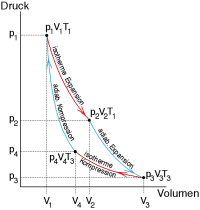
\includegraphics{pictures/carnot.png}\\

Der Wirkungsgrad einer W"armemaschine ist definiert als Verh"altnis der geleisteten Arbeit und der zugef"uhrten W"arme\\
$\epsilon=\frac{\mid W\mid}{\mid Q_W \mid}=\frac{\mid Q_W\mid - \mid Q_K \mid}{\mid Q_W \mid}=1-\frac{\mid Q_K \mid}{\mid Q_W \mid}$\\

Bei einer W"armepumpe ist der Wirkungsgrad wie folgt def:\\
$c_L=\frac{Q_K}{W}$\\\\

Der Wirkungsgrad der Carnotschen W"armemaschine\\
$\frac{Q_W}{Q_K}=\frac{T_1\ln(V_2/V_1)}{T_3\ln(V_4/V_3)}=-\frac{T_1\ln(V_2/V_1)}{T_3\ln(V_3/V_4)}=-\frac{T_1}{T_3}$\\
Der Wirkungsgrad der W"armemaschine von Carnot ist dann gleich\\
$\epsilon_{Carnot}=\frac{\mid W\mid}{\mid Q_W \mid}=1-\frac{\mid Q_K \mid}{\mid Q_W \mid}=1-\frac{T_3}{T_1}$\\\\

Der Wirkungsgrad aller zwischen zwei Temperaturen reversibel arbeitenden W"armemaschinen ist gelich gross, und alle irreversiblen W"armemaschinen haben einen kleineren Wirkungsgrad.\\
$\epsilon_{reale}<\epsilon_{Carnot}=1-\frac{T_3}{T_1}<1$\\

\subsubsection{Konzept der Irreversibilit"at}

Ein irreversibler Prozess ist ein Prozess, der nicht in umgekehrter Reihenfolge ablaufen kann.\\\\

Ein St"uck Eis wird in eine Tasse mit Wasser eingetaucht. Das Eis schmilzt. Die Temperatur des Wassers in der Tasse sinkt. Ein solcher Prozess ist irreversibel. Es gibt nur eine Richtung f"ur den Vorgang.\\

Der Prozess der freien Expansion wird als nicht reversibel bezeichnet, weil die W'keit, dass alle Gasmolek"ule sich zu einer sp"ateren Zeit wieder im ersten Volumen befinden ist extrem klein.


\section{Relativit"at}

\subsection{Transformation von einem Bezugssystem ins andere}

$t=t'$\\
$\vec{v}(t)=\frac{d\vec{R}}{dt}+\vec{v}'(t)$\\
$\vec{a}(t)=\frac{d^2\vec{R}}{dt^2}+\vec{a}(t)$

\subsection{Inertialsysteme}

Wenn die zwei Beobachter eine unterschiedliche Beschleunigung messen, kann das zweite Newtonsche Gesetz nicht f"ur beide Beobachter gelten (wenn sie beide dieselbe Kraft messen)\\

Ein Bezugssystem, in dem die Newtonschen Gesetze gelten, heisst Inertialsystem.\\

Verschiedene Inertialsysteme bewegen sich relativ zueinander mit konstanter Geschwindigkeit.\\

\subsection{Rotierendes Bezugssystem}

Winkelgeschwindigkeit:\\
$\omega(t)\equiv\frac{d\Theta(t)}{dt}$

\subsubsection{Zentrifugalkraft}
$F_{Zentrifugal}\equiv\frac{mv^2}{r}=m\omega^2 r$

\subsubsection{Corioliskraft}
$a_{Coriolis=2\omega v}$\\

$\omega_x=\omega_E\cdotp\sin(\phi_X)$\\
$\omega_X$: Winkelgeschwindigkeit mir der sich Laborsystem in X (mit geog. Breite $\phi_X$) dreht.


\subsection{Die Galileische Transformation}

O' bewegt sich mit Geschw. V in x-Richtung relativ zu O.
$x'=x-Vt$\\
$y'=y$\\
$z'=z$\\
$t'=t$
$x'=x-Vt$\\\\

Geschwindigkeitsparameter $\beta$:\\
$\beta\equiv\frac{V}{c}$\\\\

inverse Galileische Transformation von O' nach O:\\
$x=x'+Vt'=x'+\beta ct'$\\
$y=y'$\\
$z=z'$\\
$t=t'$

\subsection{Bestimmung der Lichtgeschwindigkeit}

$c=\frac{1}{\sqrt{\epsilon_0\mu_0}}=3\times10^8\:m/s$\\\\

Jeder Beobachter misst in allen Richtungen f"ur die Lichtgeschwindigkeit im Vakuum denselben Wert c.\\

D.h. die Lichtgeschwindigkeit ist gleich in alle Richtungen und unabh"angig von der Bewegung des Beobachters.

\subsection{Die Lorentz-Transformation}

Die Galileische Transformation entspricht einer N"aherung, die nur gilt, wenn die Geschw. viel kleiner als die Lichtgeschw. sind.\\\\

Lorentz-Faktor:\\
$\gamma\equiv\frac{1}{\sqrt{1-\beta^2}},\:\:\beta=\frac{v}{c}$\\

Lorentz-Transformation:\\
$x'=\gamma(x-\beta ct)$\\
$y'=y$\\
$z'=z$\\
$ct'=\gamma(ct-\beta x)$\\
x: Strecke in x-Richtung die zur"uckgelegt (+/-) beachten.

\subsection{spezielle Relativit"atstheorie}

Prinzip der Relativit"at:\\
Man kann eine gradlinige Bewegung mit konstanter Geschwindigkeit nicht f"uhlen.

\subsubsection{Raumzeitintervall $\Delta s$}

$(\Delta s)^2=(c\Delta t)^2-(\Delta x)^2-(\Delta y)^2-(\Delta z)^2$\\
Die Raumzeit ist f"ur alle Beobachter gleich.\\

$\Delta s=c\cdotp\Delta\tau$ $\Delta\tau$: Eigenzeitintervall
\subsubsection{Eigenzeit und Zeitdilatation}

Die zeitliche Entfernung zwischen zwei Ereignissen, die bez"uglich einem Bezugssystem am selben Ort stattfinden, heisst Eigenzeitintervall $\Delta\tau$.\\
$\Delta t'$ bzgl. O' gemessene Zeit, $\Delta\tau$ bzgl. O gemessene Zeit\\

$\Delta t'=\gamma\Delta\tau$

\subsubsection{L"angenkontraktion}

Die r"aumliche Entfernung zwischen zwei Punkten (oder die L"ange eines Gegenstandes) erscheint geringer, wenn sich der Beobachter relativ zu diesen Punkten bewegt als wenn er relativ zu ihnen ruht.\\
$\Delta x'$ bzgl. O' gemessene L"ange, $\Delta\lambda$ bzgl. O gemessene L"ange\\
$\Delta x'=\frac{\Delta\lambda}{\gamma}$

\subsubsection{Gleichzeitigkeit}

Werden zwei Uhren in ihrem Ruhesystem synchronisiert, so sind sie in keinem anderen Bezugssystem synchron. In dem Bezugssystem, in dem die Uhren sich bewegen, geht die f"uhrende Uhr um einen Betrag
$$\Delta t_s=l_R\frac{v}{c^2}$$
vor (zeigt eine sp"atere Zeit an), wobei $l_R$ der Ruheabstand der Uhren ist.

\subsection{Der Raumzeit 4-Vektor}

$x^\mu\equiv(ct,x,y,z)$


\subsection{Der relativistische Energie-Impuls Vektor}

Energie-Impuls 4-Vektor:\\
$p^\mu\equiv(E,\vec{p}c)$\\
$E'=\gamma m_0c^2$\\
$cp_x'=-\gamma m_0\beta c^2$\\
$cp_y'=cp_y$\\
$cp_z'=cp_z$\\\\

Ruhemasse als Invariante der Lorentz-Transformation\\
$E^2=(m_0c^2)^2+(\vec{p}c)^2$\\\\

Energie-Impulserhaltung:\\
$P^\mu=\sum_i p_i^\mu$\\
Dieser Gesamt-Energie-Impuls 4-Vektor wird erhalten, falls das System isoliert ist.

\subsection{Die Rot- und Blauverschiebung des Lichts}


\textbf{Blauverschiebung}\\
Wenn sich die Quelle in Richtung des Beobachters bewegt, wir die vom Beobachter gemessene Wellenl"ange kleiner als sie im Quellensystem erscheint. D.h., das Verh"altnis der Frequenzen ist gleich:\\
$\frac{\nu}{\nu'}=\frac{\lambda'}{\lambda}=\sqrt{\frac{1+\beta}{1-\beta}}\geq 1$\\\\

\textbf{Rotverschiebung}\\
Im Fall einer sich vom Beobachter wegbewegenden Quelle finden wir $\beta\rightarrow -\beta$\\
$\frac{\nu}{\nu'}=\frac{\lambda'}{\lambda}=\sqrt{\frac{1-\beta}{1+\beta}}\leq 1$\\\\

\textbf{Hubble-Gesetz}\\
$v=Hr$\\
v Geschw. relativ zur Erde, r die Entfernung von der Erde, und H die Hubble-Konstante\\
$H=72\pm 8 (km/s)/Mpc$

\section{Elektromagnetismus}

\subsection{Elektr. und magnetische Felder}

\subsubsection{Das elektrische Feld}

Wenn wir eine Punktladung Q und, in einem bestimmten Abstand r von ihr, eine Punktladung q betrachten, so "ubt die Punktladung Q eine Kraft auf die Punktladung q aus. Sie wirkt entlang der Verbindungslinie zwischen q und Q.\\
Die elektr. Kraft, die die Ladung Q auf eine Ladung q aus"ubt, ist gleich
$$\vec{F}=\frac{1}{4\Pi\epsilon_0}\frac{qQ}{r^2}\frac{\vec{r}}{r}$$\\

Wir definieren das elektr. Feld der Punktladung Q als
$$\vec{E}(\vec{r})\equiv\frac{\vec{F}(\vec{r})}{q}=\frac{1}{4\Pi\epsilon_0}\frac{Q}{r^2}\frac{\vec{r}}{r}$$\\


\subsubsection{Die Lorentz-Kraft}

Die allgemeine elektromagnetische Kraft wird als Funktion zweier Vektorfelder, des elektr. und des magnetischen Feldes ausgedr"uckt.\\
$$\vec{F}\equiv\vec{F}_E+\vec{F}_B=q(\vec{E}+\vec{v}\times\vec{B})$$\\
wobei E das elektr. Feld und B das magnetische Feld

$$F_B=q\vec{v}\times\vec{B}$$
$$F_L=I\vec{l}\times\vec{B}$$\\

Wir bemerken, dass
\begin{enumerate}
 \item eine Punktladung ein elektr. Feld E in jedem Punkt des Weltraums um sie erzeugt. Das elektr. Feld "ubt die elektr. Kraft qE auf eine zweite Ladung q an deren Ort aus.
 \item eine bewegte Punktladung ein magnetisches Feld B in jedem Punkt des Weltraums erzeugt. Das magnetische Feld "ubt die magnetische Kraft $qv\times B$ auf eine zweite bewegte Ladung q aus.
\end{enumerate}

Einheiten:\\
$[\vec{E}]=\frac{N}{C}$\\
$[\vec{V}]=T\:\:1T=10^4 G$\\

\textbf{Magnetische Kraft}\\
Wir bemerken, dass
\begin{enumerate}
 \item Die Kraft proportional zur Geschw. ist. Auf ein ruhendes Teilchen wirkt keine magnetische Kraft.
 \item Die Kraft senkrecht zur Bewegungsrichtung und zur Richtung des Feldes wirkt.
 \item Der Betrag der magnetischen Kraft ist gleich $|\vec{F}_B| = |q| |\vec{v}||\vec{B}| \sin \alpha$ (Lorentzkraft)
\end{enumerate}

\subsection{Feldlinien}

\subsubsection{elektr. Feldlinien}

Die Feldlinien folgen in allen Punkten des Raumes der Richtung des Feldes.\\

Regeln f"ur die elektr. Feldlinien:\\
\begin{enumerate}
 \item Die elektr. Feldlinien beginnen bei positiven Ladungen und enden bei negativen Ladungen oder im Unendlichen.
 \item Um einen einzelne Punktladung sind die Feldlinien kugelsymmetrisch verteilt.
 \item Die Anzahl der Feldlinien um eine Punktladung ist zur Gr"osse der Ladung proportional.
\end{enumerate}

\subsubsection{Magnetische Feldlinien}

Es gibt keine Punkte im Raum, an denen die magnetischen Feldlinien anfangen oder enden. Deshalb bilden die magnetischen Feldlinien geschlossene Schleifen.\\

Die Feldlinien zeigen immer von N nach S.\\

Die Wechselwirkung zwischen gleichen Magnetpolen ist abstossend, die zwischen ungleichen Polen anziehend.

\subsection{Elektr. potentielle Energie und elektr. Potential}

Wir betrachten zwei Ladungen q und Q im Abstand r voneinander, die elektr. pot. Energie ist gleich:
$$E^e_{pot}(\vec{r})=\frac{1}{4\Pi\epsilon_0}\frac{qQ}{r}$$\\

Das elektr. Potential wird definiert als:
$$V(\vec{r})\equiv\frac{E^e_{pot}(\vec{r})}{q}$$

Wir k"onnen daher den elektr. Potentialunterschied zwischen zwei Punkten als die Arbeit definieren, die ein elektr. Feld leistet, wenn es eine Einheitsladung von einem Punkt zu einem anderen bewegt.\\

\subsubsection{Potentialdifferenz}
$$\Delta V =V_b-V_a=\frac{\Delta E_{pot}}{q}=\int^b_a Edl$$

Kinetische Energie, die eine Ladung q gewinnt, wenn sie durch eine Potentialdifferenz $\Delta V$ beschleunigt wird:
$\Delta E_{kin}=|q\Delta V|$\\

Einheit:\\
$[V]=J/C=V$

\subsubsection{Kontinuierliche Ladungsverteilung}

$$V=\int\limits_V \frac{1}{4\pi\epsilon_0}\frac{dq}{r}$$

Bei einer kontinuierlichen Ladungsverteilung findet man das Potential durch Integration "uber die Ladungsverteilung.

\subsubsection{Der Gradient des Potentials}

Das elektr. Feld ist der negative Gradient des elektr. Potentials:\\
$\vec{E}=-\vec{\nabla}V$\\
Einheit des elektr. Feldes:\\
$[\vec{E}]=N/C=V/m$

\subsubsection{elektr. Potential des elektr. Dipols}

$V(r)\approx\frac{q}{4\Pi\epsilon_0}(\frac{a\cos\theta}{r^2})$

\subsubsection{elektr. Spannung}

$U_{AB}\equiv V(\vec{r}_A)-V(\vec{r}_B)$


\subsection{Elektr. Strom}

$I(t)\equiv \frac{dQ}{dt}$\\
wobei dQ die Ladungsmenge ist, die in der Zeit dt durch die Fl"ache A tritt. Man benutzt die historische Konvention, dass die positive Stromrichtung der Flussrichtung der positiven Ladungen folgt.\\
Einheit $1 A = 1 C/s$\\\\

Driftgeschw. $v_D$, bei Dichte der beweglichen Ladungstr"ager gleich n:
$I\frac{\Delta Q}{\Delta t}=\frac{qn(Av_D\Delta t)}{\Delta t}=qnAv_D$

\subsubsection{Die Stromdichte und die Leitf"ahigkeit}

Stromdichte j:\\
$j=\frac{I}{A}=\sigma E$\\
wobei $\sigma$ die Leitf"ahigkeit des Leiters ist. Die Stromdichte ist zum elektr. Feld proportional.\\
Einheit: $[\sigma]=\frac{A}{Vm}$\\
Ohm $\Omega=\frac{V}{A}$

\subsubsection{Das Ohmsche Gesetz}

$U=RI=(\frac{L}{\sigma A}I)$\\
R: Widerstand des Leiters, L: L"ange

\subsubsection{Die elektr. Leistung}

$P=UI=RI^2$

\subsubsection{Spezifischer Widerstand}

$R=\rho\frac{l}{A}$

\subsection{Berechnung der elektr. und magnetischen Felder}

Raumladungsdichte $\rho$:\\
$\rho(\vec{r})\equiv \frac{dq}{dV}$\\
Fl"achenladungsdichte $\sigma$:\\
$\sigma\equiv\frac{dq}{dA}$\\
Linienladungsdichte $\lambda$:\\
$\lambda\equiv\frac{dq}{dl}$\\\\

\subsubsection{Berechnung des E-Feldes}


Coulomb-Gesetz:\\
Eine Punktladung dq erzeugt ein elektr. Feld in einem bestimmten Punkt r gleich\\
$d\vec{E}(\vec{r})=\frac{1}{4\Pi\epsilon_0}\frac{dq}{r^3}\vec{r}$\\
Wobei sich die Ladung im Ursprung des Koordinatensystems befindet.\\
Wenn sich die Ladung in einem Punkt r' befindet, dann ist das E-Feld gleich:\\
$d\vec{E}(\vec{r})=\frac{1}{4\Pi\epsilon_0}\frac{dq}{\mid \vec{r} -\vec{r}' \mid^3}(\vec{r}-\vec{r}')$\\\\

F"ur eine kontinuierliche Ladungsverteilung ($dq=\rho dV$), gilt:\\
$\vec{E}(\vec{r})=\int\int\int\frac{1}{4\Pi\epsilon_0}\frac{\rho(\vec{r}')}{\mid \vec{r} -\vec{r}' \mid^3}(\vec{r}-\vec{r}')d^3\vec{r}'$\\\\

F"ur einen unendlichen Stab gilt:\\
$\mid \vec{E} \mid=\frac{2\lambda}{4\Pi\epsilon_0}\frac{1}{r}$


\subsubsection{Berechnung des B-Feldes (Bio-Savart)}

Eine Punktladung q, die sich mit der Geschwindigkeit v bewegt, erzeugt im Raum ein Magnetfeld B, das gegeben ist durch
$$B=\frac{\mu_0}{4\pi}\frac{qv\times r/r}{r^2}$$

Das Feld in einem Punkt r ist gleich:\\
$d\vec{B}(\vec{r})=\frac{\mu_0}{4\Pi}\frac{dq}{r^2}(\vec{v}\times\frac{\vec{r}}{r})$\\

Das Feld das durch das Stromelement $Idl$ erzeugt wird, ist gleich
$(dq)\vec{v}=(\frac{dq}{dt})(\vec{v}dt)=I\vec{dl}$\\
$d\vec{B}(\vec{r})=\frac{\mu_0}{4\Pi}\frac{I}{r^2}(d\vec{l}\times\frac{\vec{r}}{r})$\\

$\vec{B}(\vec{r})=\int d\vec{B}$

\subsection{Bewegte Ladungen in elektr. und magnetischen Feldern}

\subsubsection{Bewegung einer Punktladung in einem elektr. Feld}

$\vec{F}=q\vec{E}=m\vec{a}\:\Rightarrow\:\vec{a}=\frac{q}{m}\vec{E}$\\
oft m"ussen wir die relativistische Masse benutzen:\\
$\vec{a}=\frac{q}{\gamma m_0}\vec{E}$


\subsubsection{Bewegung einer Punktladung in einem magnetischen Feld}

Zyklotron:\\
$\omega=\frac{qB}{\gamma m_0}$\\
$T=\frac{2\Pi}{\omega}=\frac{2\Pi\gamma m_0}{qB}$\\
$f=\frac{1}{T}=\frac{qB}{2\Pi\gamma m_0}$


\subsection{Kraft auf einen elektr. Strom}

Ein elektr. Strom besteht aus einer Ansammlung sich bewegender Ladungen. Wir erwarten daher, dass ein Magnetfeld auch auf einen Leiter durch den ein Strom fliesst, eine Ablenkungskraft aus"ubt. Die Gesamtkraft auf einen Leiter der Querschnittsfl"ache A und L"ange L ist.\\
$\vec{F}=L\vec{I}\times \vec{B}$\\

f"ur ein differentielles Element des Stroms:\\
$d\vec{F}=Ld\vec{I}\times \vec{B}=Id\vec{L}\times\vec{B}$

\subsection{Der Fluss und die Divergenz des Flusses}

Der Fluss $d\phi$ eines Vektorfeldes F durch eine infinitesimale Fl"ache $dA$ wird definiert als (der Fluss ist eine Skalargr"osse):\\
$$d\phi\equiv \vec{F}\cdotp d\vec{A}=\mid \vec{F}\mid\mid d\vec{A}\mid \cos \theta$$
wobei dA ein Vektor ist, der dem infintesimalen Fl"achenelement dA entspricht.\\

F"ur eine endliche Fl"ache von beliebiger Form wird der Fluss durch Integration der infintesimalen ebenen Fl"achenelemente gewonnen. Der gesamte Fluss durch die Oberfl"ache A ist deshalb gleich
$$\phi\equiv \iint\limits_A \vec{F}\cdotp d\vec{A}$$
(Integration "uber die Fl"ache A)\\

H"aufig sind wir am Fluss durch eine \textit{geschlossene} Oberfl"ache interessiert. Definitionsgem"ass zeigen in diesem Fall die infinitesimalen Fl"achen dA an jedem Punkt der Oberfl"ache nach aussen.
$$\phi\equiv\oiint\limits_{geschlossene\:A}\vec{F}\cdotp d\vec{A}$$


\subsubsection{Der elektr. und magnetische Fluss}

$\phi_E \equiv \iint\limits_A \vec{E}\cdotp d\vec{A}$ (Elektr. Fluss)\\
$\phi_B \equiv \iint\limits_A \vec{B}\cdotp d\vec{A}$ (Magn. Fluss)\\

\subsubsection{Die Divergenz des Feldes}

Die Divergenz des Feldes in jedem Punkt (x,y,z) ist gleich dem Fluss, der das Volumenelement im Punkt (x,y,z) des Volumens dxdydz verl"asst pro Volumeneinheit.\\
$d\phi_{tot}(x,y,z)=(\vec{\nabla}\cdotp\vec{F}(x,y,z))dxdydz$\\
wobei wir den Nabla-Operator f"ur die Divergenz des Feldes im Punkt (x,y,z) verwendet haben.\\
$\vec{\nabla}\cdotp\vec{F}(x,y,z)=(\frac{\partial F(x,y,z)}{\partial x}\frac{\partial F(x,y,z)}{\partial y}\frac{\partial F(x,y,z)}{\partial z})$\\\\

\textbf{Theorem der Divergenz/ Theorem v. Gauss}\\
Theorem der Divergenz f"ur den gesamten Fluss $\phi_{tot}$ der ein Volumen V verl"asst:
$$\phi_{tot}\equiv \oiint\limits_{A=\partial V}\vec{F}\cdotp d\vec{A}=\iiint\limits_{V}(\vec{\nabla}\cdotp\vec{F})dV$$
wobei A die Oberfl"ache ist, die das Volumen V umschliesst.

\subsection{Das Gauss'sche Gesetz}

Gesetz von Gauss f"ur das elektr. Feld:\\
$\epsilon_0(\vec{\nabla}\cdotp \vec{E}(\vec{r}))=\rho(\vec{r})$\\

Diese Beziehung zwischen der Divergenz des elektr. Feldes und der Ladungsdichte in jedem Punkt des Raumes entspricht einem fundamentalen Gesetz des Elektromagnetismus.\\\\

Es folgt daraus:\\
$\phi_{tot}\equiv\oiint\limits_{A=\partial V}\vec{E}\cdotp d\vec{A}=\iiint\limits_{V}(\vec{\nabla}\cdotp\vec{E})dV=\frac{1}{\epsilon_0}\iiint\limits_{V}\rho(\vec{r})dV=\frac{Q_{innerhalb}}{\epsilon_0}$

\subsection{Divergenz des magnetischen Feldes}

Es wird nie magnetischer Fluss erzeugt oder vernichtet. Es gibt keine Punkte im Raum, an denen die magnetischen Feldlinien anfangen oder enden.\\\

Die Divergenz des magnetischen Feldes muss deshalb in jedem Punkt des Raumes gleich null sein:
$$\vec{\nabla}\cdotp\vec{V}(\vec{r})=0$$
Gesetz von Gauss f"ur das magnetische Feld\\


\subsection{Stromdichte und Ladungserhaltung}

Wenn die gesamte Ladung, die im Volumen V enthalten ist, sich "andert, muss ein Strom durch die Oberfl"ache des Volumens fliessen.\\
Die zeitliche "Anderung der gesamten Ladung innerhalb des Volumens ist deshalb gleich dem Strom, der durch die Obefl"ache des Volumens fliesst:\\
$-\frac{dQ}{dt}=I(t)$\\
Wir verwenden nun die Stromdichte j(r), so dass die Summe der Stromdichte "uber eine endliche Fl"ache A gleich der gesamten Stromst"arke ist, die durch die Fl"ache A fliesst:\\
$I\equiv\iint\limits_{A}\vec{j}(\vec{r})\cdotp d\vec{A}$\\
Die Stromdichte ist die Stromst"arke pro Fl"acheneinheit. Die Stromst"arke durch eine ebene Fl"ache dA ist gleich\\
$i_A=\vec{j}\cdotp d\vec{A}$\\
Einheit: $[\vec{j}]=\frac{A}{m^2}$\\\\

Kontinuit"atsgleichung:\\
$\frac{\partial \rho(\vec{r})}{\partial t}+\vec{\nabla}\cdotp\vec{j}(\vec{r})=0$\\
Diese Gleichung gilt in jedem Punkt des Raumes. Sie sagt, dass wenn sich die Ladung in einem Punkt "andert, in diesem Punkt ein elektr. Strom fliessen muss.

\subsection{Das Linienintegral eines Feldes}

\subsubsection{Theorem von Stokes}

$\oint\limits_{C=\partial A}\vec{F}\cdotp d\vec{r}=\iint\limits_{A}(\vec{\nabla}\times\vec{F}\cdotp d\vec{A})$\\

Wenn die Rotation des Feldes in jedem Punkt des Raumes verschwindet, ist das Linienintegral vom Punkt A zum Punkt B unabh"angig vom Weg. In diesem Fall ist das Feld \textbf{konservativ} (oder ein Potentialfeld).

\subsection{Das Ampersche Gesetz}

$\oint\limits_{C}\vec{B}d\vec{r}=\mu_0 I_C$\\
Wobei $I_C$ der Strom ist, der durch die Fl"ache hindurchtritt, die durch die Kurve begrenzt wird. \\\\

Es muss in jedem Punkt des Raumes gelten:\\
$(\vec{\nabla}\times\vec{B})(\vec{r})=\mu_0\vec{j}(\vec{r})$\\
Gesetz von Ampere f"ur das magnetische Feld\\
Wobei $j(r)$ die Stromdichte und $\mu_0$ die magnetische Feldkonstante ist.

\subsection{Maxwellsche Gleichungen}

Die Maxwellschen Gleichungen fassen in einer kompakten mathematischen Formulierung die beiden Gesetze von Gauss f"ur das elektr. und magnetische Feld sowie die Gesetze von Ampere zusammen.\\
Zus"atzlich wurden auch das sogenannte Gesetz von Faraday und eine Erweiterung des Gesetzes von Ampere, die mit der zeitlichen "Anderung  der Felder zu tun hat, von Maxwell hinzugef"ugt.\\\\

$\epsilon_0(\vec{\nabla}\cdotp\vec{E})=\rho$\\
$(\vec{\nabla}\cdotp\vec{B})=0$\\
$\vec{\nabla}\times\vec{E}=-\frac{\partial\vec{B}}{\partial t}$\\
$\vec{\nabla}\times \vec{B}=\mu_0\vec{j}+\epsilon_0\mu_0\frac{\partial\vec{E}}{\partial t}$\\\\

Im Fall der Elektrostatik und Megnetostatik sind die Felder von der Zeit unabh"angig, und die Gleichungen vereinfachen sich zu:\\

$\epsilon_0(\vec{\nabla}\cdotp\vec{E})=\rho$\\
$(\vec{\nabla}\cdotp\vec{B})=0$\\
$\vec{\nabla}\times\vec{E}=0$\\
$\vec{\nabla}\times \vec{B}=\mu_0\vec{j}$\\\\


Aus den urspr"unglichen zeitabh"angigen Gleichungen folgt eine wichtige physikalische Regel:\\
Ein zeitver"anderliches magnetisches (bzw. elektr.) Feld erzeugt ein elektr. (bzw. magnetisches) Feld.


\subsection{Gesetz von Faraday (Induktionsgesetz)}


$U_{induziert}=\oint\limits_{C=\partial A}\vec{E}\cdotp d\vec{r}=-\frac{d}{dt}\iint\limits_{A}\vec{B}\cdotp d\vec{A}=-\frac{d\phi_B}{dt}$\\
wobei $\phi_B$ der magnetische Fluss durch die Fl"ache A ist, und C die Kurve, die die Fl"ache A einschliesst.\\\\

Wenn die Leiterschleife einen geschlossenen Stromkreis bildet, werden sich die beweglichen Elektronen in der Schleife bewegen. Man spricht von induziertem Strom. Im Falle von Metallen kann man das Ohmsche Gesetz benutzen:\\
$I_{induziert}=U_{induziert}/R=-\frac{1}{R}\frac{d\phi_B}{dt}$\\\\

Lenzsche Regel:\\
die induzierten Str"ome sind so gerichtet, dass sie ihrer Ursache, d.h. der "Anderung des magnetischen Flusses entgegenwirken.\\
Richtung gegeben durch die Richtung der magn. Kraft auf eine \textit{positive} Ladung.


\section{Elektromagnetische Wellen}

\subsection{Felder eines bewegten geladenen Drahtes}

$|\vec{B}|=(\epsilon_0\mu_0 v)|\vec{E}|=(\epsilon_0\frac{1}{\epsilon_0 c^2}v)|\vec{E}|=(\frac{v}{c^2}|\vec{E}|)$

\subsection{Die elektromagnetischen Wellen}

Im Allgemeinen werden elektromagnetische Wellen erzeugt, wenn geladene Teilchen beschleunigt werden.

\subsubsection{Wellengleichung und Ausbreitungsgeschw.}

Laplace-Operator:\\
$\vec{\nabla}\cdotp\vec{\nabla}=\vec{\nabla}^2=\frac{\partial^2}{\partial x^2}+\frac{\partial^2}{\partial y^2}+\frac{\partial^2}{\partial z^2}$\\\\

Wellengleichung der elektromagnetischen Wellen:\\
$\vec{\nabla}^2\vec{E}=\epsilon_0\mu_0\frac{\partial^2\vec{E}}{\partial t^2}$ und $\vec{\nabla}^2\vec{B})=\epsilon_0\mu_0\frac{\partial^2\vec{B}}{\partial t^2}$\\
Die Ausbreitungsgeschwindigkeit der Welle ist gleich c.\\\\

Die Beziehung zwischen den Betr"agen der Felder ist die folgende:\\
$|\vec{B}|=(\frac{v}{c^2})|\vec{E}|=\frac{1}{c}|\vec{E}|$ oder $|\vec{E}|=c|\vec{B}|$

\subsubsection{F"ur eine elektromagnetische Welle im Vakuum (Luft) gilt}

\begin{itemize}
 \item $|\vec{E}|=c|\vec{B}|\rightarrow B_0=\frac{1}{c}E_0$
 \item $\vec{E}\perp\vec{B}$
 \item $\vec{E},\vec{B}\perp\vec{v}$ (Ausbreitungsrichtung)\\
  $\vec{E}\times\vec{B}$ zeigt in Ausbreitungsrichtung\\
  $\rightarrow\:\vec{E},\vec{B},\vec{v}$ bilden ein Rechtssystem
 \item wegen $|\vec{E}|=c|\vec{B}|$ schwingen $\vec{E}$ und $\vec{B}$ in Phase
  z.B. ist f"ur $E_x=E_y=0,E_z=E_0\sin(ky-\omega t)$ und Bewegungsrichtung y-Achse\\
  $B_y=B_z=0\:B_x=B_0\sin(ky-\omega t),\:B_0=\frac{1}{c}E_0$
\end{itemize}

\subsection{Ebene Wellen}

\subsubsection{Harmonische}

$\vec{k}\equiv(k_x,k_y,k_z)=Wellenvektor$\\

Die Felder einer ebenen, elektromagnetischen Welle werden dann geschrieben als:\\
$\vec{E}(\vec{r},t)=\vec{E}_0\sin(\vec{k}\cdotp\vec{r}-\omega t)$\\
$\vec{B}(\vec{r},t)=\vec{B}_0\sin(\vec{k}\cdotp\vec{r}-\omega t)$\\
wobei $E_0$ und $B_0$die Amplitudenvektoren sind. Sie besitzen einen Betrag und eine Richtung, die der Polarisation der Welle entspricht.\\
$\omega = \mid \vec{k} \mid c$\\
Wellenzahl $|k|=\frac{2\pi}{\lambda}$\\\\

Die Felder m"ussen senkrecht zur Ausbreitungsrichtung sein:\\
$\vec{k}\cdotp\vec{E}_0=\vec{k}\cdotp\vec{B}_0=0\:\Rightarrow\: \vec{k}\perp\vec{E}_0$ und $\vec{k}\perp\vec{B}_0$\\\\

Und mit Hilfe der Maxwellschen Gl. gilt:\\
$\vec{B}=(\vec{k}\times\vec{E}_0)\frac{1}{\omega}\sin(\vec{k}\cdotp\vec{r}-\omega t)=\frac{1}{\omega}(\vec{k}\times\vec{E})$

\subsection{Das elekromagnetische Spektrum}

$c=\lambda \nu$\\
$E=h\nu$

\subsection{Die Polarisation}

Wir definieren die Polarisation der Welle als die Richtung des elektrischen Feldes.\\\\

Der Polarisator: es gibt bestimmte Platten aus einem polarisierenden Material, die nur die Wellen hindurchlassen, deren Polarisation parallel zu einer bestimmten Transmissionsrichtung sind. Die Wellen, die senkrecht zu dieser Richtung polarisiert sind, werden von der Platte absorbiert.\\\\

Gesetz von Malus:\\
Wenn der Winkel zwischen den Transmissionsrichtungen gleich $\theta$ ist, ist die Intensit"at der durchgelassenen Welle\\
$I=I_0\cos^2\theta$\\
wobei $I_0$ das Maximum der hindurchgelassenen Intensit"at ist.

\subsection{Energie und Impuls der elektromagnetischen Wellen}

Energiestromdichte (od. Leistungsdichte) der Welle:\\
Einheit: $\frac{W}{m^2}$

\subsubsection{Poynting-Vektor}

$\vec{S}\equiv\frac{1}{\mu_0}\vec{E}\times\vec{B}$\\
Dieser Vektor zeigt in die Richtung, in die Energie transportiert wird.\\
$[\vec{S}]=\frac{J}{m^3}\frac{m}{s}$\\\\

F"ur eine harmonische Welle gilt:\\
$I=\frac{1}{2\mu_0 c}E_0^2=\frac{\epsilon_0}{2}E_0^2c\:\:[\frac{Watt}{m^2}]$

\subsubsection{Intensit"at als Funktion der Distanz}

Ein Beobachter befindet sich in einer Entfernung r von einer Punktquelle der Energie pro Zeiteinheit (= Strahlungsleistung) $P_0$.\\

$E_0=\frac{1}{r}\sqrt{\frac{P_0\mu_0 c}{2\Pi}}$ und $B_0=E_0/c$

\subsubsection{Elektromagnetischer Druck}

Wir betrachten eine elektromagnetische Welle, die auf eine Fl"ache f"allt und vollst"andig absorbiert wird. Wir nehmen an, dass die absorbierte Energie (w"ahrend einem Zeitintervall) gleich E ist.\\
$p_{em-Druck}=\frac{E}{c}$\\
$E=I\cdotp t\cdotp A\rightarrow\langle F \rangle=\frac{P}{t}$\\
$[p]=[Impuls]=kg\cdotp\frac{m}{s}$\\
Wird die Welle vollst"andig von der Fl"ache reflektiert, so ist der "ubertragene Impuls doppelt so gross:\\
$p_{em-Druck}=\frac{2E}{c}$

\subsubsection{Leistung}

$P=A\cdotp I$

\subsection{Wellentheorie der elektromagnetischen Wellen}

\subsubsection{Prinzip von Huygens}

Jeder Punkt einer Wellenfront kann als Ausgangspunkt f"ur eine kugelf"ormige Elementarwelle betrachtet werden.

\subsubsection{Reflexion und Brechung}

F"allt ein Lichtstrahl auf eine Oberfl"ache, so wird er dort sowohl reflektiert als auch gebrochen.\\

Der Einfallwinkel $\theta_1$, der Reflexionswinkel $\theta_1'$ und der Brechungswinkel $\theta_2$ werden relativ zur Normalen der Grenzoberfl"ache definiert.

  \begin{picture}(100,100)
   \put(0,50){\line(1,0){100}}
   \multiput(50,0)(0,1){100}{\line(0,1){0.7}} 
   \put(0,100){\line(1,-1){50}}
   \put(50,50){\line(1,1){50}}
   \put(50,50){\line(1,-2){20}}
   
   \put(57,20){\makebox(0,0){$\theta_2$}}
   \put(40,75){\makebox(0,0){$\theta_1$}}
   \put(60,75){\makebox(0,0){$\theta_1'$}}

   \put(30,65){\makebox(0,0){Medium 1}}
   \put(30,35){\makebox(0,0){Medium 2}}
  \end{picture}

Es gilt:\\
\begin{enumerate}
 \item Der reflektierte und der gebrochene Strahl liegen in der vom einfallenden Strahl und der Normale der Grenzfl"ache gebildeten Ebene.
 \item Reflexionsgesetz:\\
  $\theta_1=\theta_1'$
 \item Brechungsgesetz:\\
  $\frac{\sin\theta_1}{\sin\theta_2}=n_{21}$
 \item $n_1\sin\theta_1=n_2\sin\theta_2$
\end{enumerate}

Wobei $n_{21}$ die Brechzahl des Mediums 2 gegen das Medium 1 ist.


\subsubsection{Totalrefelxion}

F"ur Einfallswinkel gr"osser als dieser Grenzwinkel $\theta_g$ existiert kein gebrochener Strahl mehr.\\
$\frac{\sin\theta_g}{\sin90}=\sin\theta_g=\frac{n_2}{n_1}$ mit $n_2>n_1$

\subsubsection{Beugung an einem Spalt}

Wir betrachten eine ebene Welle der Wellenl"ange $\lambda$, die auf einen Spalt mit der Breite a f"allt. $a\approx \lambda$\\
Nach dem Prinzip von Huygens wirkt jeder Punkt des Spaltes als eine Quelle einer sich ausbreitenden Elementarwelle. Weil die Breite des Spaltes ungef"ahr so gross wie die Wellenl"ange ist, entspricht der Spalt einer einzelnen Quelle.\\
Es folgt daraus, dass die ebene Welle die auf den Spalt f"allt, sich nachher als konzentrische Kreise ausbreiten wird.

\subsubsection{Ausbreitung des Lichtes durch einen Einzelspalt}
Erstes Minimum:\\
$\frac{a}{2}\sin\theta = \frac{\lambda}{2}\:\Rightarrow\:a\sin\theta=\lambda$\\

Kein Minimum, falls $a\ll\lambda$, da $\sin\theta=\frac{\lambda}{a}\rightarrow\infty$\\

Beugung verschwindet, falls $a\gg\lambda$\\

\subsubsection{Beugung am Doppelspalt}

d: Abstand zw. den Spalten\\
$\Delta x$: Gangunterschied\\

$\Delta x =\frac{2\Pi n}{k}=n\lambda\:\:n=0,1,2,\ldots$\\

Damit im Punkt P ein Maximum der Intensit"at entsteht, muss gelten:\\
$\Delta x=d\sin\theta=n\lambda\:\:\:n=0,1,2,\ldots$\\

und f"ur Minima:\\
$\Delta x=d\sin\theta=(n+\frac{1}{2})\lambda\:\:\:n=0,1,2,\ldots$\\

\subsection{R"ontgenbeugung}

Licht f"allt auf die Oberfl"ache eines Kristalls. Das Gitter soll eine kubische Symmetrie aufweisen.\\
a: Abst. zw. 2 benachbarten Atomen\\
Es gilt: $\theta_{einfallende}=\phi_{gebeugte}$


\appendix
 \section{Physikalische Konstanten}
  \footnotesize
  \begin{tabular}{l l l}
   Gravitationskonstante &	G &				$6.67\cdotp 10^{-11}\:\frac{Nm^2}{kg^2}$\\
   Lichtgeschwindigkeit &	c &				$3\cdotp 10^8\:\frac{m}{s}$\\
   Magnetische Feldkonstante &	$\mu_0$	&			$4\Pi\cdotp 10^{-7}\:\frac{Vs}{Am}$\\
   Elektr. Feldkonstante &	$\epsilon_0=1/\mu_0 c^2$ &	$8.854\cdotp 10^{-12}\:\frac{As}{Vm}$\\
   Elementarladung &		e &				$1.602\cdotp 10^{-19}\:C$\\
   Plancksches Wirkungsquant. &	h &				$6.602\cdotp 10^{-34}\:Js$\\
   &				$\hbar=h/2\Pi$ &		$1.0546\cdotp 10^{-34}\:Js$\\
   Ruhemasse Elektron &		$m_e$ &				$9.109\cdotp 10^{-31}\:kg$\\
   Ruhemasse Proton &		$m_p$ &				$1.6726\cdotp 10^{-27}\:kg$\\
   Ruhemasse Neutron &		$m_n$ &				$1.6749\cdotp 10^{-27}\:kg$\\
   Boltzmann Konstante &	$k$ &				$1.381\cdotp 10^{-23}\:\frac{J}{K}$\\
   Univ. Gaskonstante &		$R$ &				$8.314\:J/mol/K$
  \end{tabular}
  \normalsize
 \section{Trigonometrie}
  \begin{picture}(200,95)
   \put(20,20){\line(1,0){180}}
   \put(20,20){\line(0,1){60}}
   \put(20,80){\line(3,-1){180}}
   
   \put(15,45){\makebox(0,0){b}}
   \put(100,5){\makebox(0,0){a}}
   \put(120,50){\makebox(0,0){c}}

   \put(170,25){\makebox(0,0){$\beta$}}
   \put(30,68){\makebox(0,0){$\alpha$}}
  \end{picture}
  $\sin\alpha =\frac{a}{c}=\cos\beta\:\:\:\cos\alpha =\frac{b}{c}=\sin\beta$\\
  $\tan\alpha =\frac{a}{b}=\cot\beta\:\:\:\cot\alpha =\frac{b}{a}=\tan\beta$

\end{document}
